\documentclass[AMA,STIX1COL]{WileyNJD-v2}
\usepackage{moreverb}
% just for todo notes
\setlength {\marginparwidth }{2cm}
\usepackage[colorinlistoftodos]{todonotes}

\newcommand\BibTeX{{\rmfamily B\kern-.05em \textsc{i\kern-.025em b}\kern-.08em
T\kern-.1667em\lower.7ex\hbox{E}\kern-.125emX}}

\articletype{Article Type}%

\received{<day> <Month>, <year>}
\revised{<day> <Month>, <year>}
\accepted{<day> <Month>, <year>}

%\raggedbottom

\begin{document}

\title{A demonstration of the \LaTeX\ class file for Wiley NJD Journals\protect\thanks{This is an example for title footnote.}}

\author[1,2]{Damon M. Bayer}

\author[2]{Michael P. Fay*}

\author[3]{Barry I. Graubard}

\authormark{D. M. BAYER, M.P. FAY and B. I. Graubard \textsc{et al}}


\address[1]{\orgdiv{Biostatistics Research Branch}, \orgname{National Institute of Allergy and Infectious Diseases}, \orgaddress{\state{Bethesda, Maryland}}}

\address[2]{\orgdiv{Department of Statistics}, \orgname{University of California, Irvine}, \orgaddress{\state{Irvine, California}, \country{Country name}}}

\address[3]{\orgdiv{Division of Cancer Epidemiology and Genetics}, \orgname{National Cancer Institute}, \orgaddress{\state{Rockville, Maryland}}}

\corres{*Michael P. Fay, Bethesda, MD 2089. \email{mfay@niaid.nih.gov}}

\presentaddress{Present address}

\abstract[Abstract]{This paper describes the use of the \LaTeXe\ \textsf{WileyNJD-v2.cls}
class file for setting papers for \emph{Mathematical Methods in the Applied Sciences}.}

\keywords{Class file; \LaTeXe; \emph{Wiley NJD}}

\jnlcitation{\cname{%
\author{Williams K.}, 
\author{B. Hoskins}, 
\author{R. Lee}, 
\author{G. Masato}, and 
\author{T. Woollings}} (\cyear{2016}), 
\ctitle{A regime analysis of Atlantic winter jet variability applied to evaluate HadGEM3-GC2}, \cjournal{Q.J.R. Meteorol. Soc.}, \cvol{2017;00:1--6}.}

\maketitle

\footnotetext{\textbf{Abbreviations:} ANA, anti-nuclear antibodies; APC, antigen-presenting cells; IRF, interferon regulatory factor}

\section{Introduction}

\section{Methods}
\todo[inline]{I’m struggling a bit with the overall message of the paper.

In Part 1, we advocate for the Kalish Appendix aka the Korn-Graubard + CD method over the Lang-Reiczigel method in the case of a simple random sample / unweighted survey. This is sort of a special case of the / Korn-Graubard + CD method with k = 1 and the binomial variance assumption, rather than the Poisson variance assumption. 

In Part 2, we advocate for Fay-Feuer over Korn-Graubard in the case where
 }
Suppose we have a survey with  \( k \) sampling units, with \( N_1, N_2, \ldots, N_k \) individuals in the population of unit \( i \).
We sample \( n_1, n_2, \ldots, n_k \) individuals via a simple random sample from each population to have an assay performed to determine who has a disease.
Let \( \theta_i \) be the population frequency of positive results for assays performed on individuals from sampling unit \( i \) and \( X_i \) be the number of positive results from an assay performed on \( n_i \) individuals from sampling unit \( i \).
Also let \( \theta_i^* \) be the population frequency of cases in sampling unit \( i \) and \( X_i^* \) be the true number of people with the disease among the \( n_i \) individuals from sampling unit \( i \).
Then \( X_i^* \sim \operatorname{Binomial}(n_i, \theta_i^*) \)
In the case of a perfect assay, \( \theta_i = \theta_i^* \) and \( X_i = X_i^* \).

Therefore, the population prevalence is 

\begin{equation}
    \beta = \frac{\sum_{i=1}^k N_i \theta_i^*}{\sum_{j=1}^k N_j} = \sum_{i=1}^k w_i \theta_i^*,
\end{equation}

where \( w_i = N_i / N \).

Suppose the assay is measured on \( m_n \) individuals known to not have the disease and on \( m_p \) individuals known to have have the disease.
Let \( C_n \) and \( C_p \) be the number who test positive from the respective samples.
Assume that the negative and positive controls act like simple random samples from their respective populations and that \( C_n \sim \operatorname{Binomial}(m_n, \phi_n) \) and \( C_p \sim \operatorname{Binomial}(m_p, \phi_p) \), where \( 1 - \phi_n \) is the specificity of the assay and \( \phi_p \) is the sensitivity of the assay.

Let \( \hat{AP} = \frac{\sum_{i=1}^k N_i \frac{X_i}{n_i}}{\sum_{j=1}^k N_j} = \sum_{i=1}^k w_i \frac{X_i}{n_i} \), \( \widehat{Sp} = 1 - \frac{C_n}{m_n} \), and \( \widehat{Se} = \frac{C_p}{m_p} \).

The first method in this paper is concerned with estimating \( \beta \) in the case where \( k = 1 \), \( \phi_n > 0 \), \( \phi_p < 1 \), i.e. estimating prevalence from a simple random sample with an imperfect assay.
The second method in this paper is concerned with estimating \( \beta \) in the case where \( k > 1 \), \( \phi_n = 0 \), \( \phi_p = 1 \), i.e. estimating prevalence from a weighted sample with a perfect assay.
The final method in this paper is concerned with estimating \( \beta \) in the case where \( k > 1 \), \( \phi_n > 0 \), \( \phi_p < 1 \), i.e. estimating prevalence from a weighted sample with an imperfect assay.

\subsection{Estimating Prevalence from a Simple Random Sample with an Imperfect Assay}

First, we consider the scenario \( k = 1 \), \( \phi_n > 0 \), \( \phi_p < 1 \) and we are concerned with estimating 

\begin{equation}
    \beta = \frac{\sum_{i=1}^k N_i \theta_i^*}{\sum_{j=1}^k N_j} = \theta_1^*
\end{equation}

We use the method is described in the Appendix of \cite{Kali:2021}.
This is a modification of the melding method, which uses lower and upper confidence distributions on functions of estimators independent estimators to create a confidence interval for prevalence that accounts for variability in \( \widehat{AP} \), \( \widehat{Se} \), and \( \widehat{Sp} \) \cite{FayP:2015}.

For each of \( \widehat{AP} \), \( \widehat{Se} \), and \( \widehat{Sp} \), we use the lower and upper confidence distributions associated with the exact binomial confidence interval.
In the case of a binomial random variable with \( x \) successes among \( n \) trials, the lower confidence distribution is \( \operatorname{Beta}(x, n - x + 1) \), and the upper confidence distribution is \( \operatorname{Beta}(x + 1, n - x) \).

Letting \( B_{ap}^L, B_{ap}^U, B_{sp}^L, B_{sp}^U, B_{se}^L, B_{se}^U \) be the lower and upper confidence distribtuions associate with the estimators, and \( q(a, W) \) be the \( a \)th quantile of a random variable \( W \), the 95\% confidence interval for \( \beta \) is 


\( \left\{ q \left( 0.025, \frac{B_{ap}^L + B_{sp}^L - 1}{B_{se}^U + B_{sp}^L - 1}  \right),  q \left( 0.975, \frac{B_{ap}^U + B_{sp}^U - 1}{B_{se}^L + B_{sp}^U - 1}  \right) \right\}.\)

This method is compared to the method presented in \citet{Lang:2014}.

\subsection{Estimating Prevalence from a Weighted Sample with a Perfect Assay}



\subsection{Estimating Prevalence from a Weighted Sample with an  Imperfect Assay}

\section{Results}
\subsection{Estimating Prevalence from a Simple Random Sample with an Imperfect Assay}
\subsection{Estimating Prevalence from a Weighted Sample with a Perfect Assay}

\begin{figure}
    \centering
    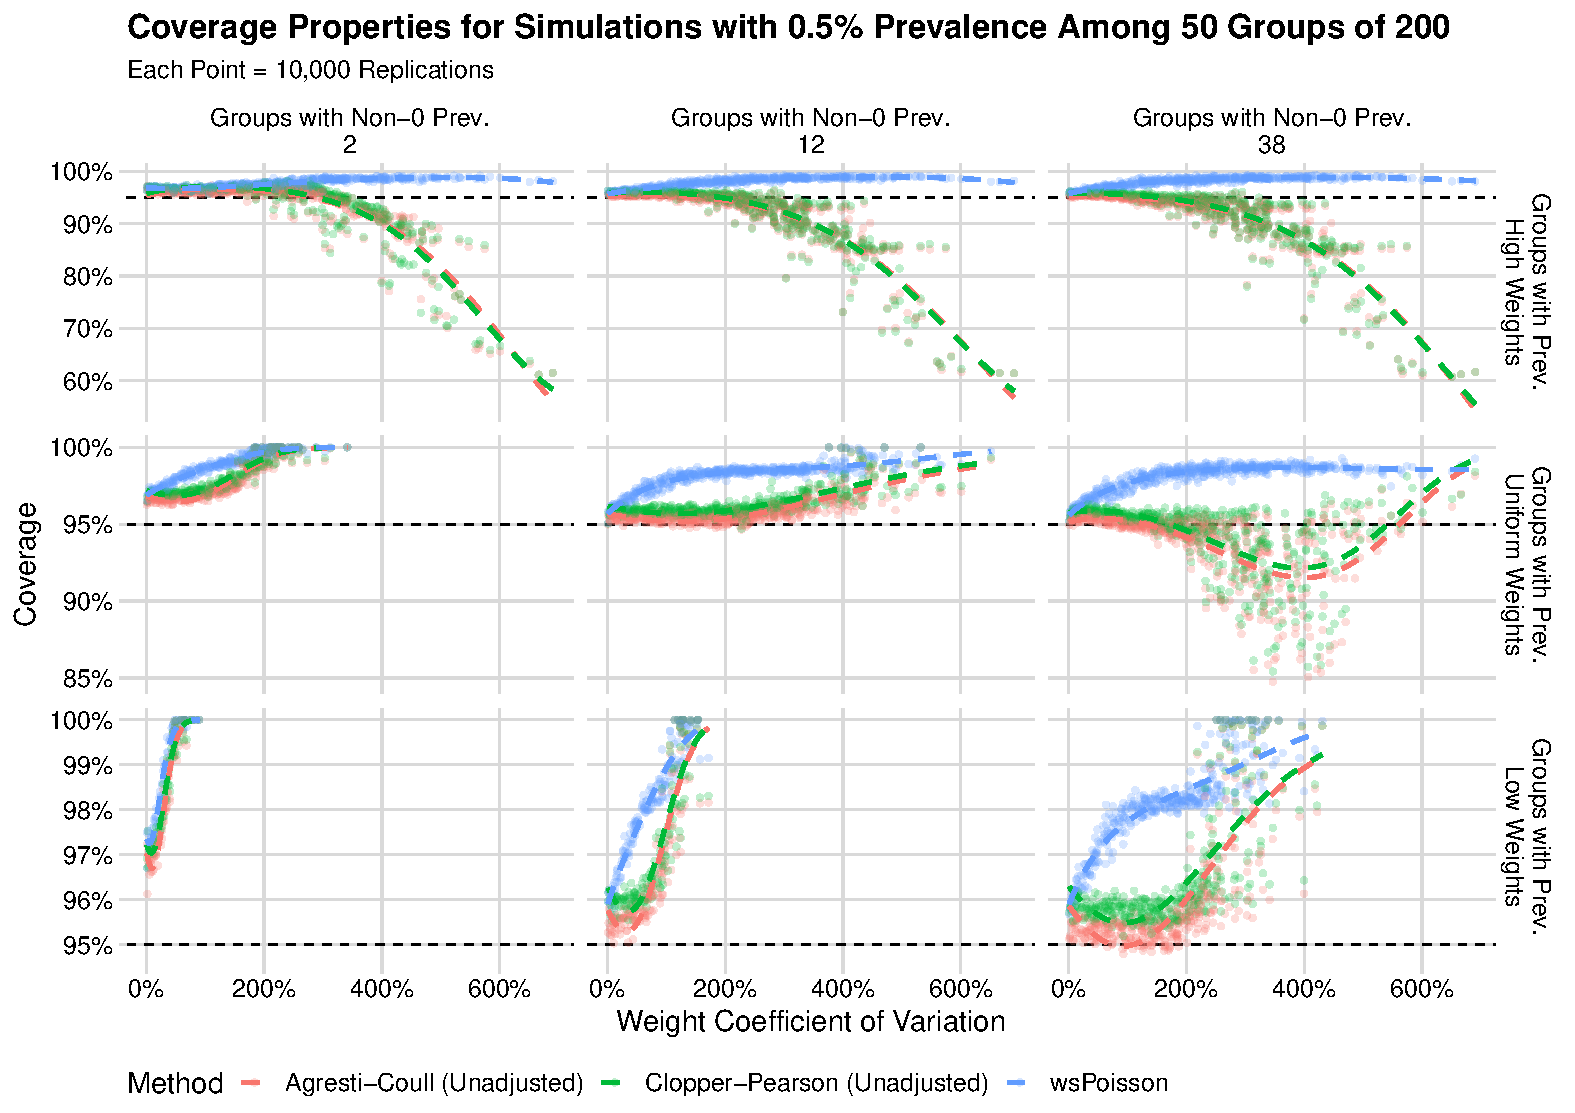
\includegraphics[width=\textwidth]{figures/perfect_coverage_50_0_005_reduced.pdf}
    \caption{Caption}
    \label{fig:perfect_coverage_50_0_005_reduced}
\end{figure}


\begin{figure}
    \centering
    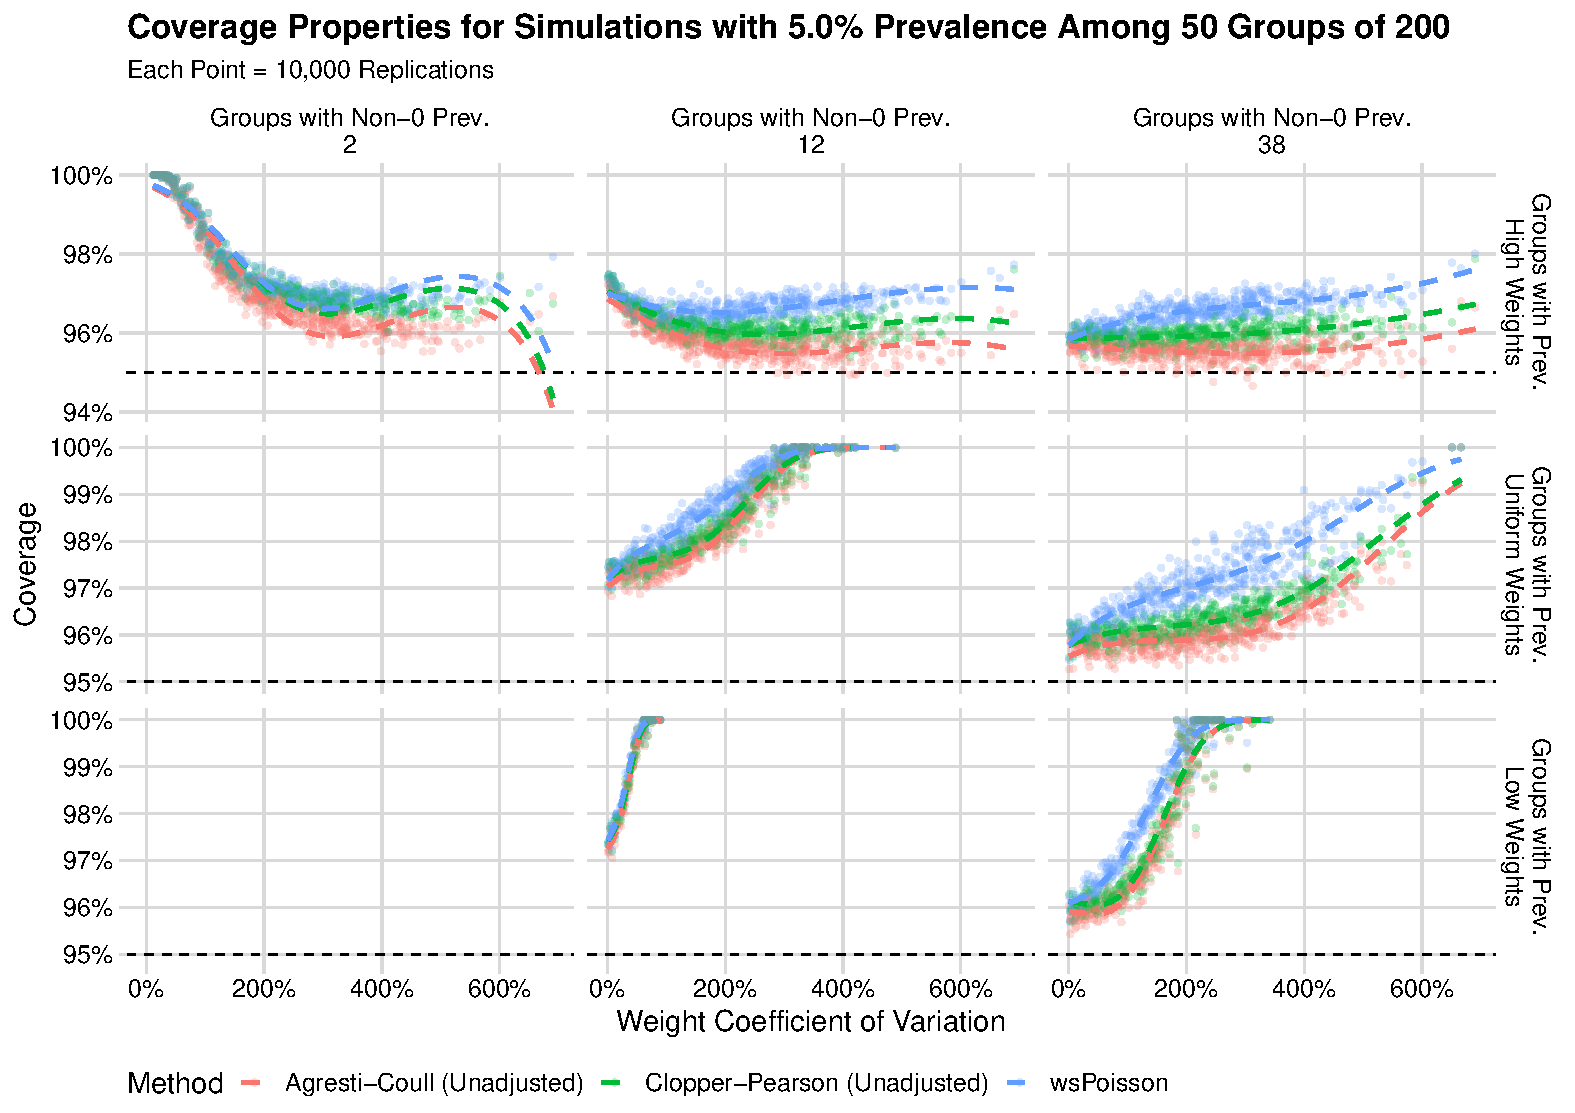
\includegraphics[width=\textwidth]{figures/perfect_coverage_50_0_05_reduced.pdf}
    \caption{Caption}
    \label{fig:perfect_coverage_50_0_05_reduced}
\end{figure}


\begin{figure}
    \centering
    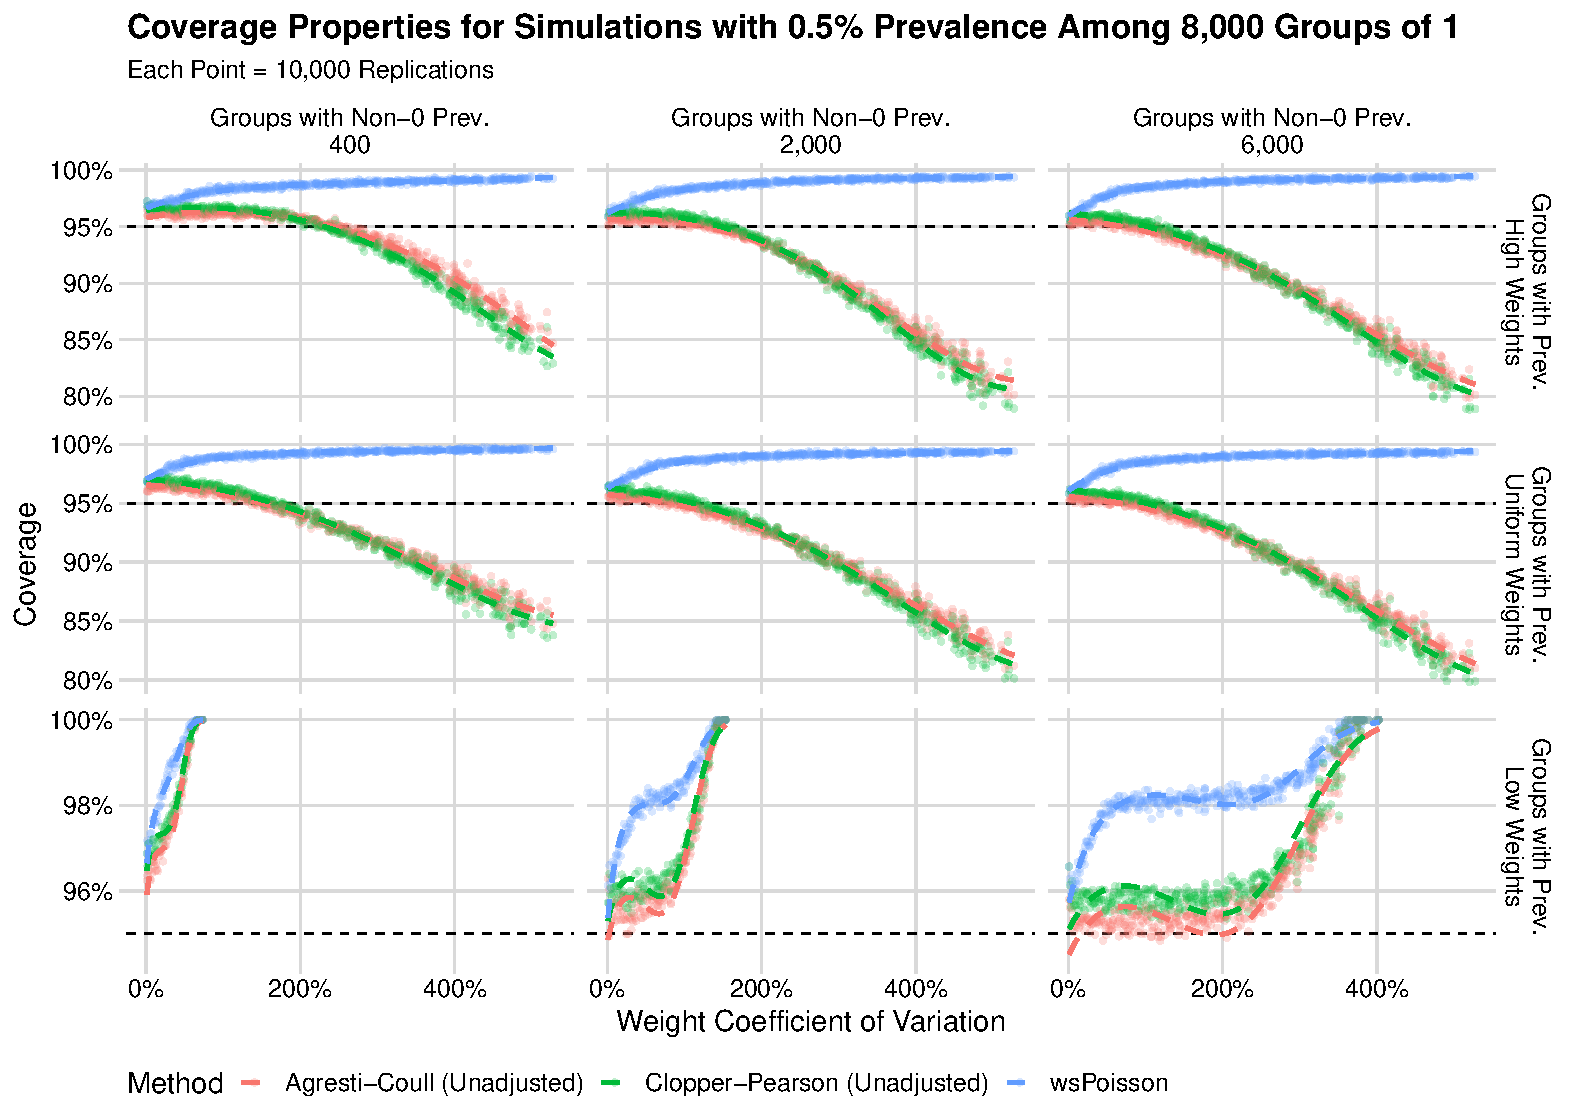
\includegraphics[width=\textwidth]{figures/perfect_coverage_8000_0_005_reduced.pdf}
    \caption{Caption}
    \label{fig:perfect_coverage_8000_0_005_reduced}
\end{figure}

\begin{figure}
    \centering
    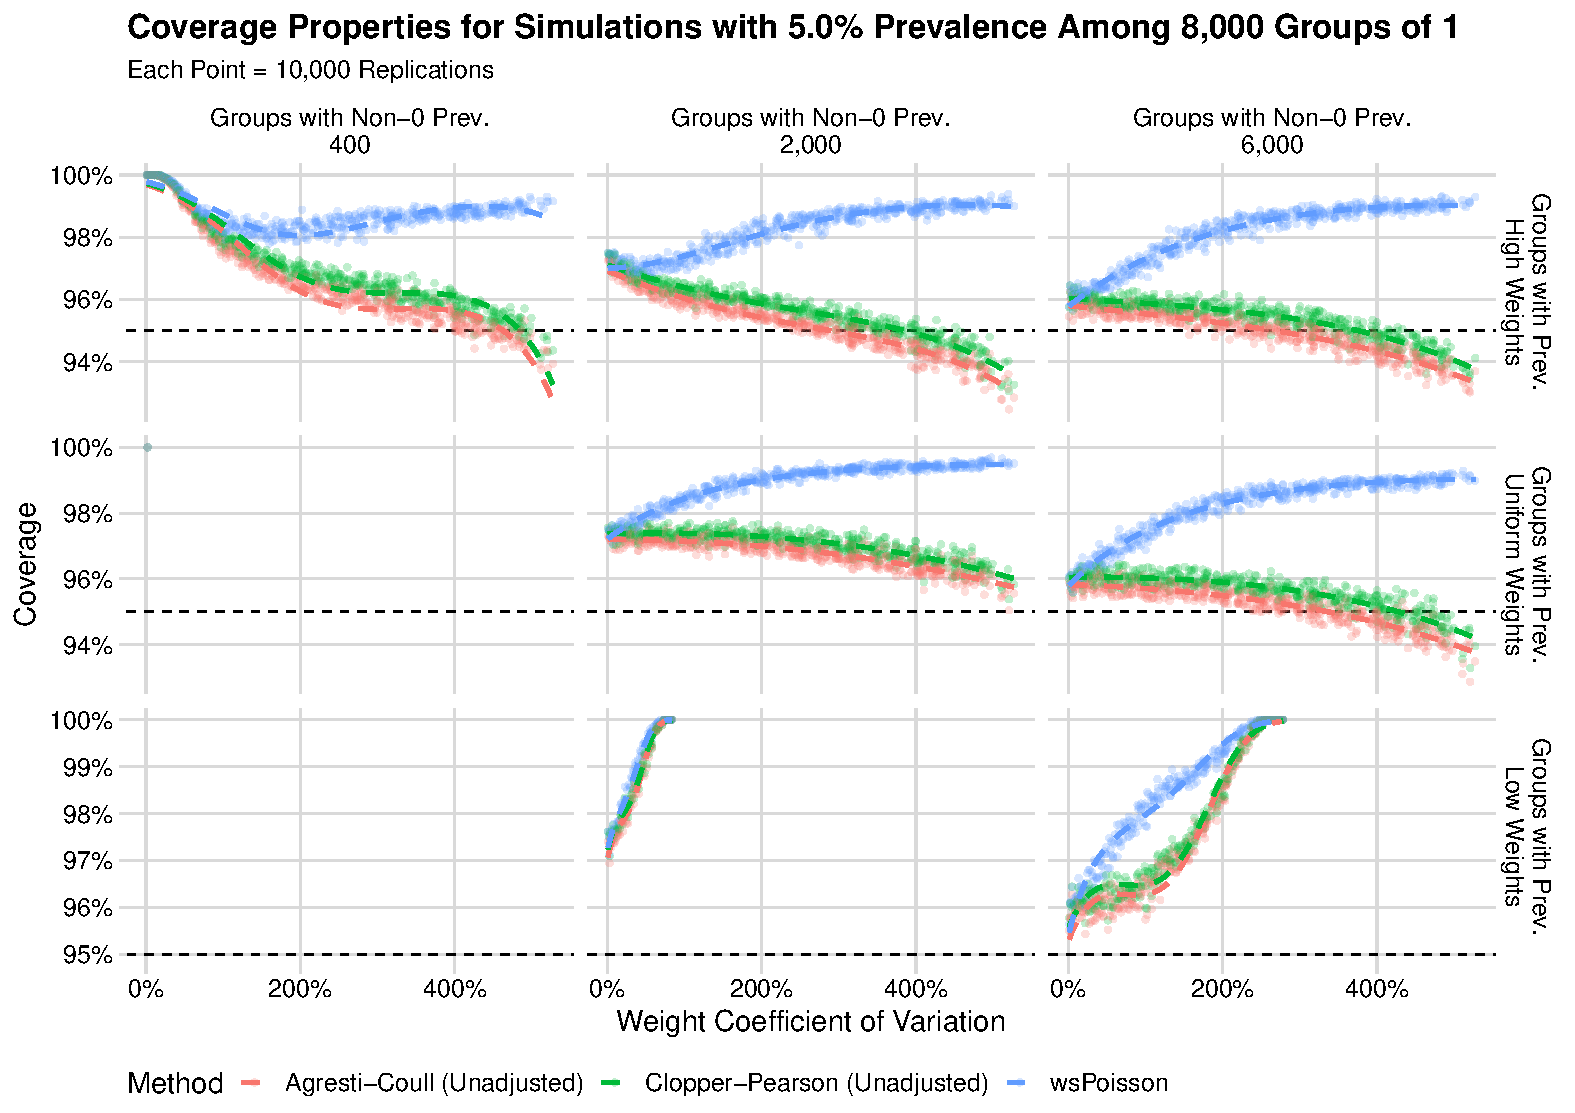
\includegraphics[width=\textwidth]{figures/perfect_coverage_8000_0_05_reduced.pdf}
    \caption{Caption}
    \label{fig:perfect_coverage_8000_0_05_reduced.pdf}
\end{figure}


\begin{figure}
    \centering
    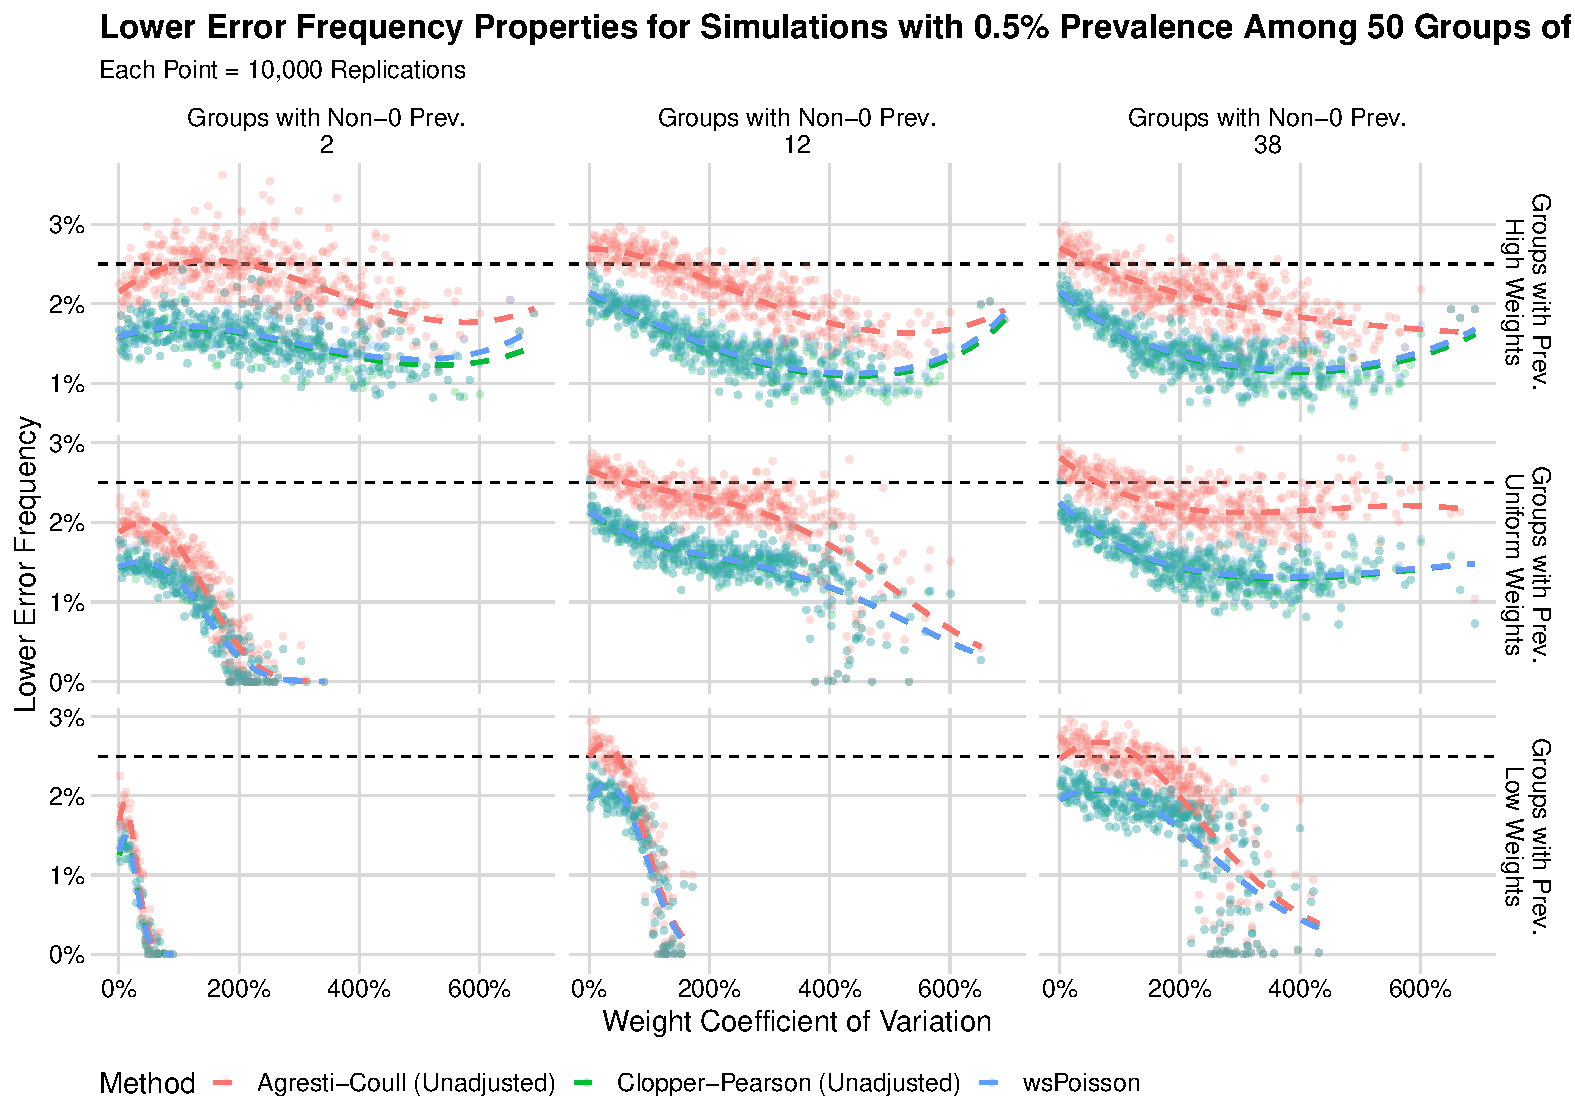
\includegraphics[width=\textwidth]{figures/perfect_lower_error_frequency_50_0_005_reduced.pdf}
    \caption{Caption}
    \label{fig:perfect_lower_error_frequency_50_0_005_reduced}
\end{figure}


\begin{figure}
    \centering
    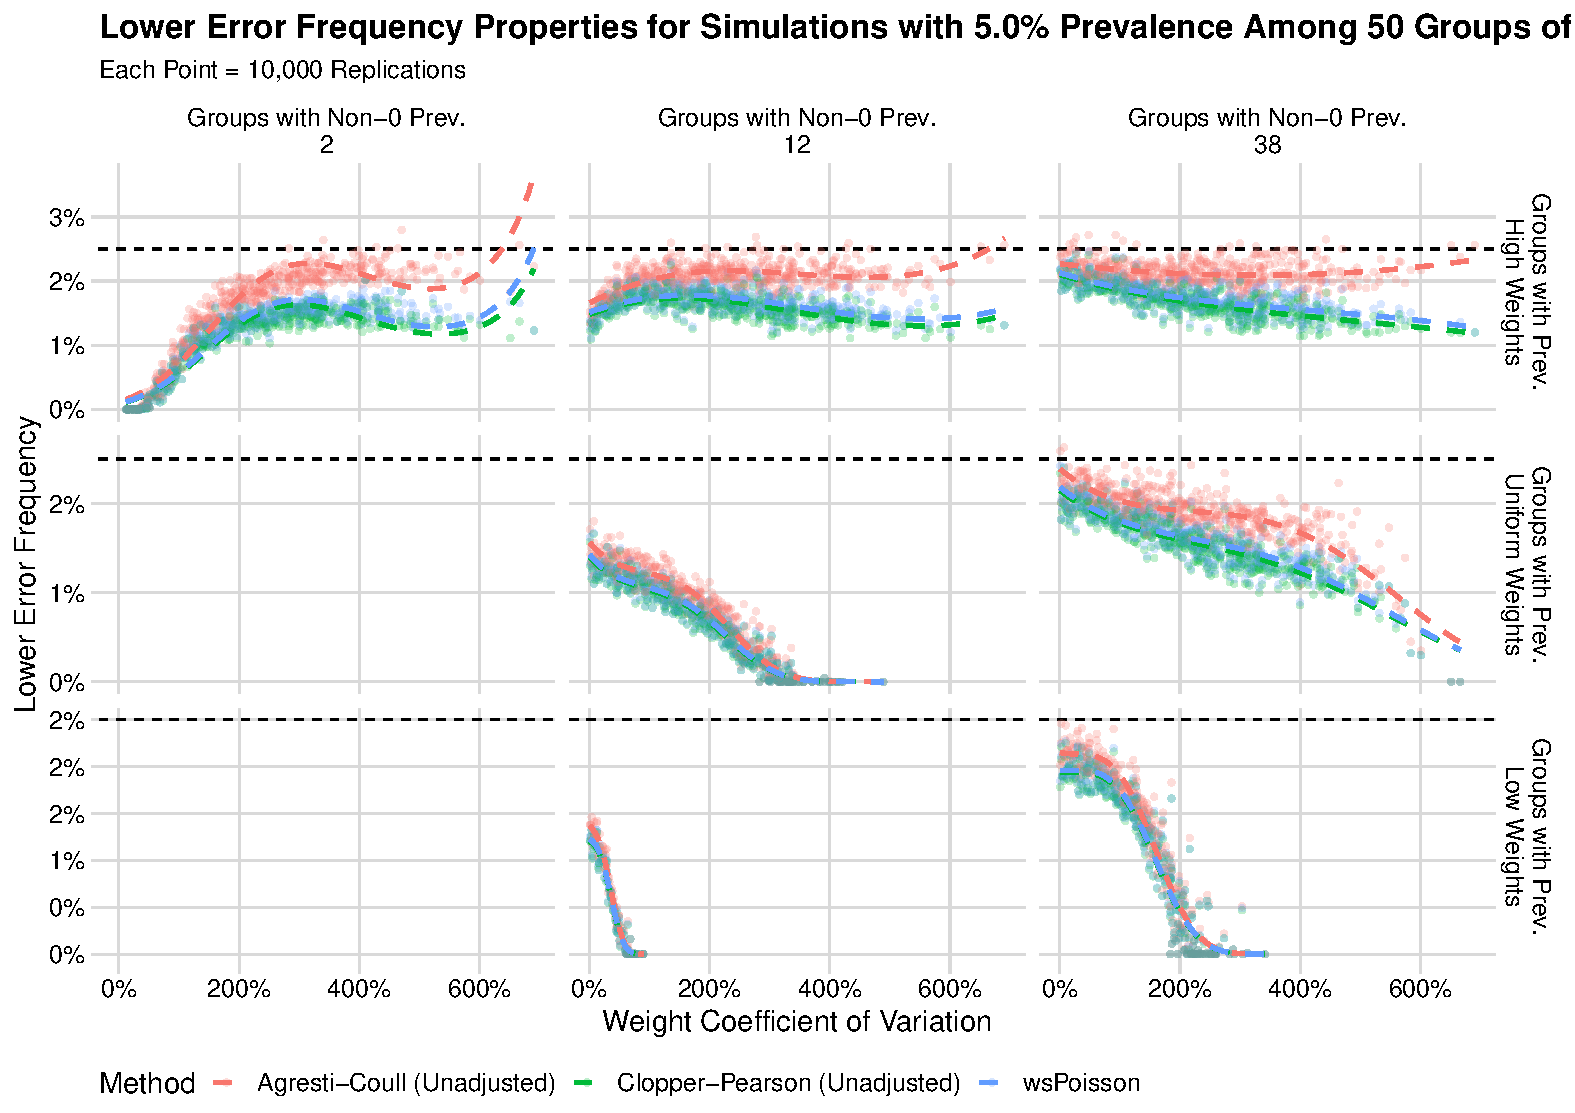
\includegraphics[width=\textwidth]{figures/perfect_lower_error_frequency_50_0_05_reduced.pdf}
    \caption{Caption}
    \label{fig:perfect_lower_error_frequency_50_0_05_reduced}
\end{figure}


\begin{figure}
    \centering
    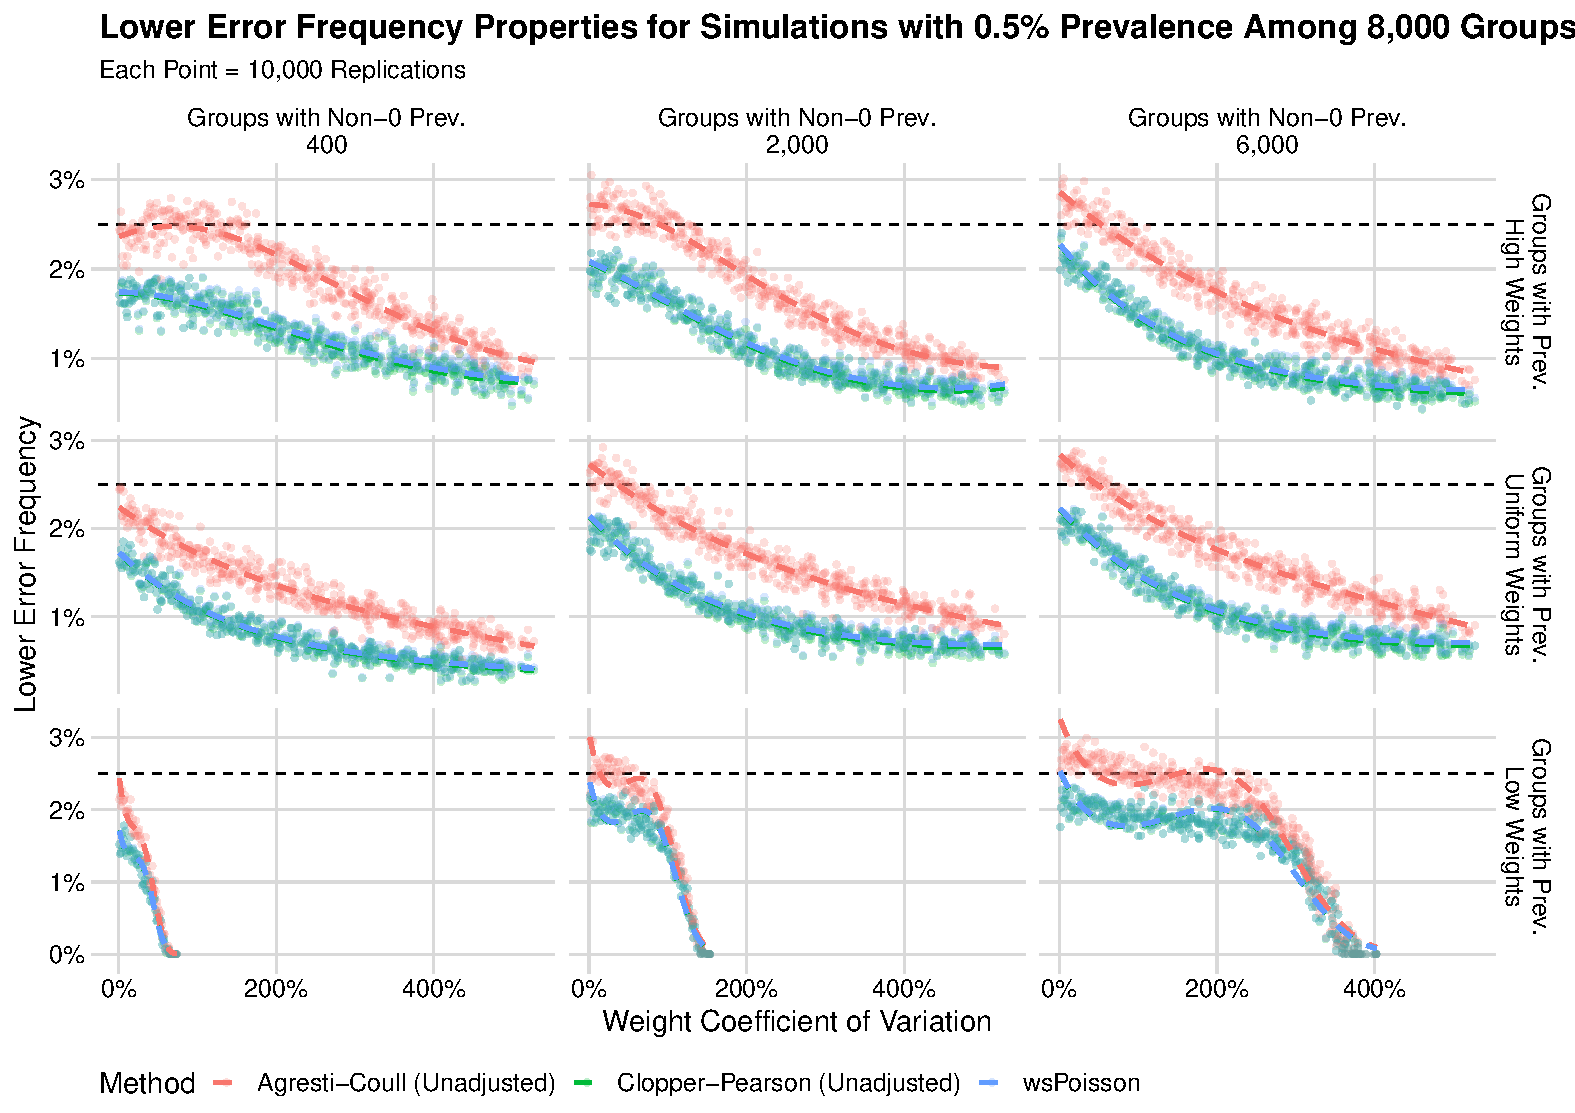
\includegraphics[width=\textwidth]{figures/perfect_lower_error_frequency_8000_0_005_reduced.pdf}
    \caption{Caption}
    \label{fig:perfect_lower_error_frequency_8000_0_005_reduced}
\end{figure}

\begin{figure}
    \centering
    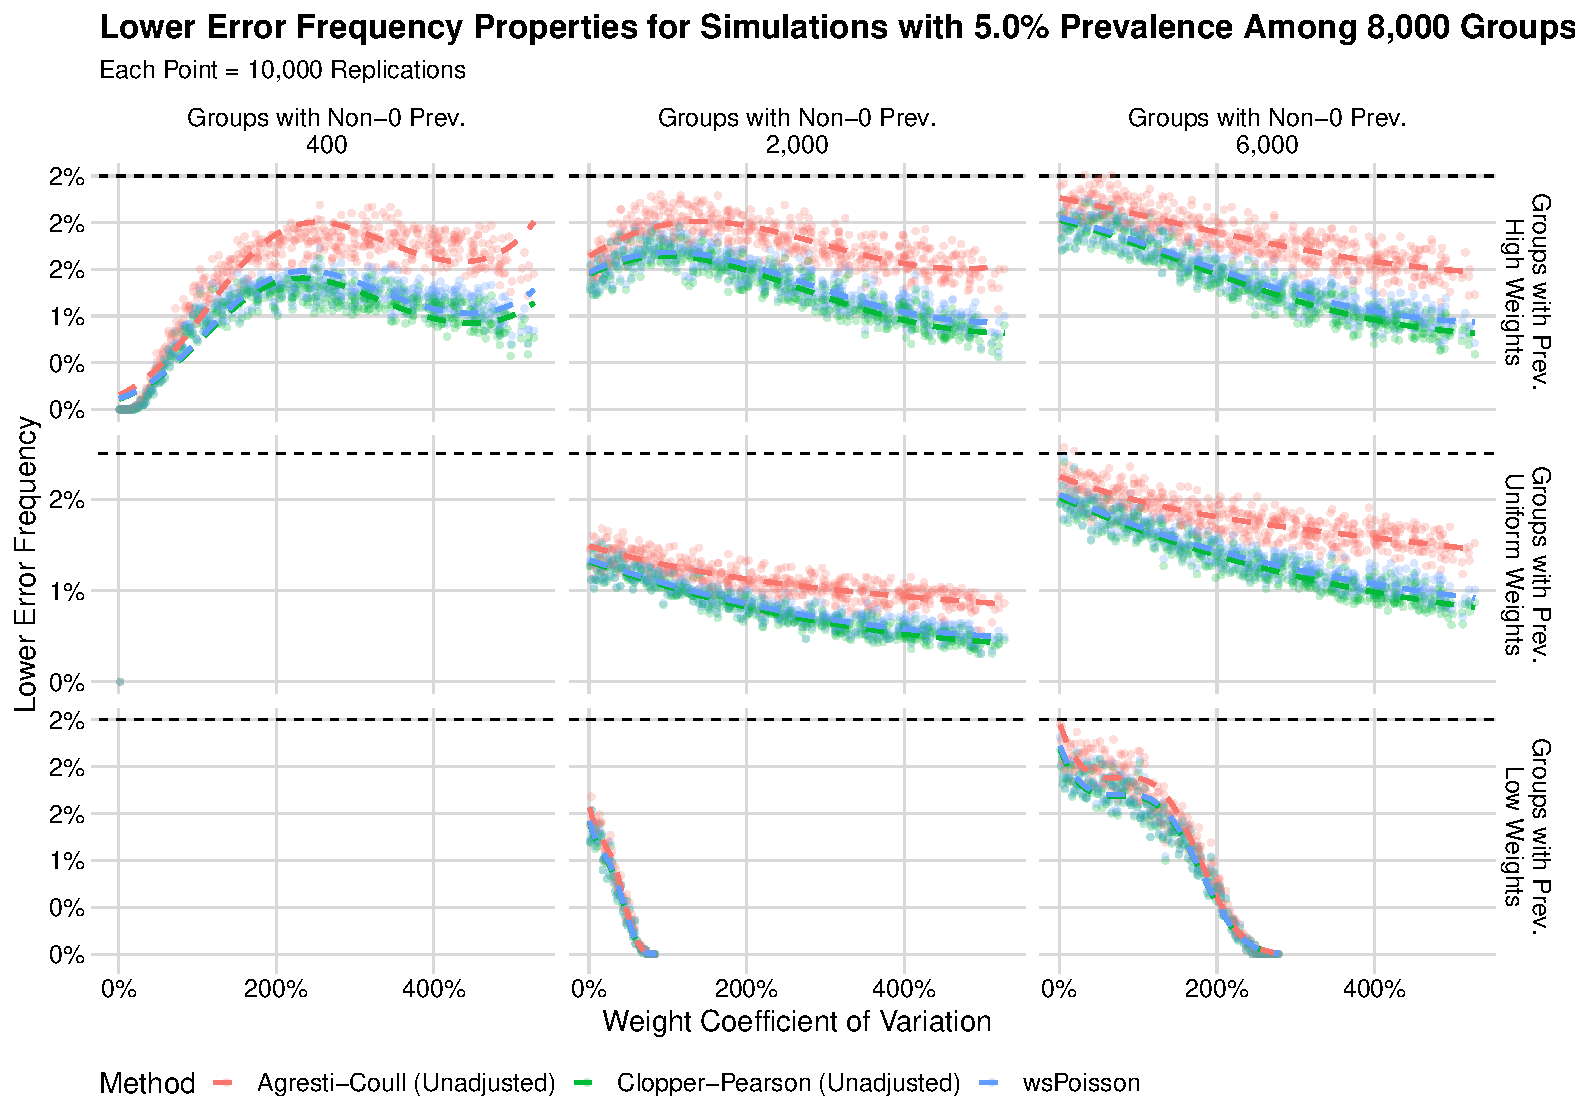
\includegraphics[width=\textwidth]{figures/perfect_lower_error_frequency_8000_0_05_reduced.pdf}
    \caption{Caption}
    \label{fig:perfect_lower_error_frequency_8000_0_05_reduced.pdf}
\end{figure}

\begin{figure}
    \centering
    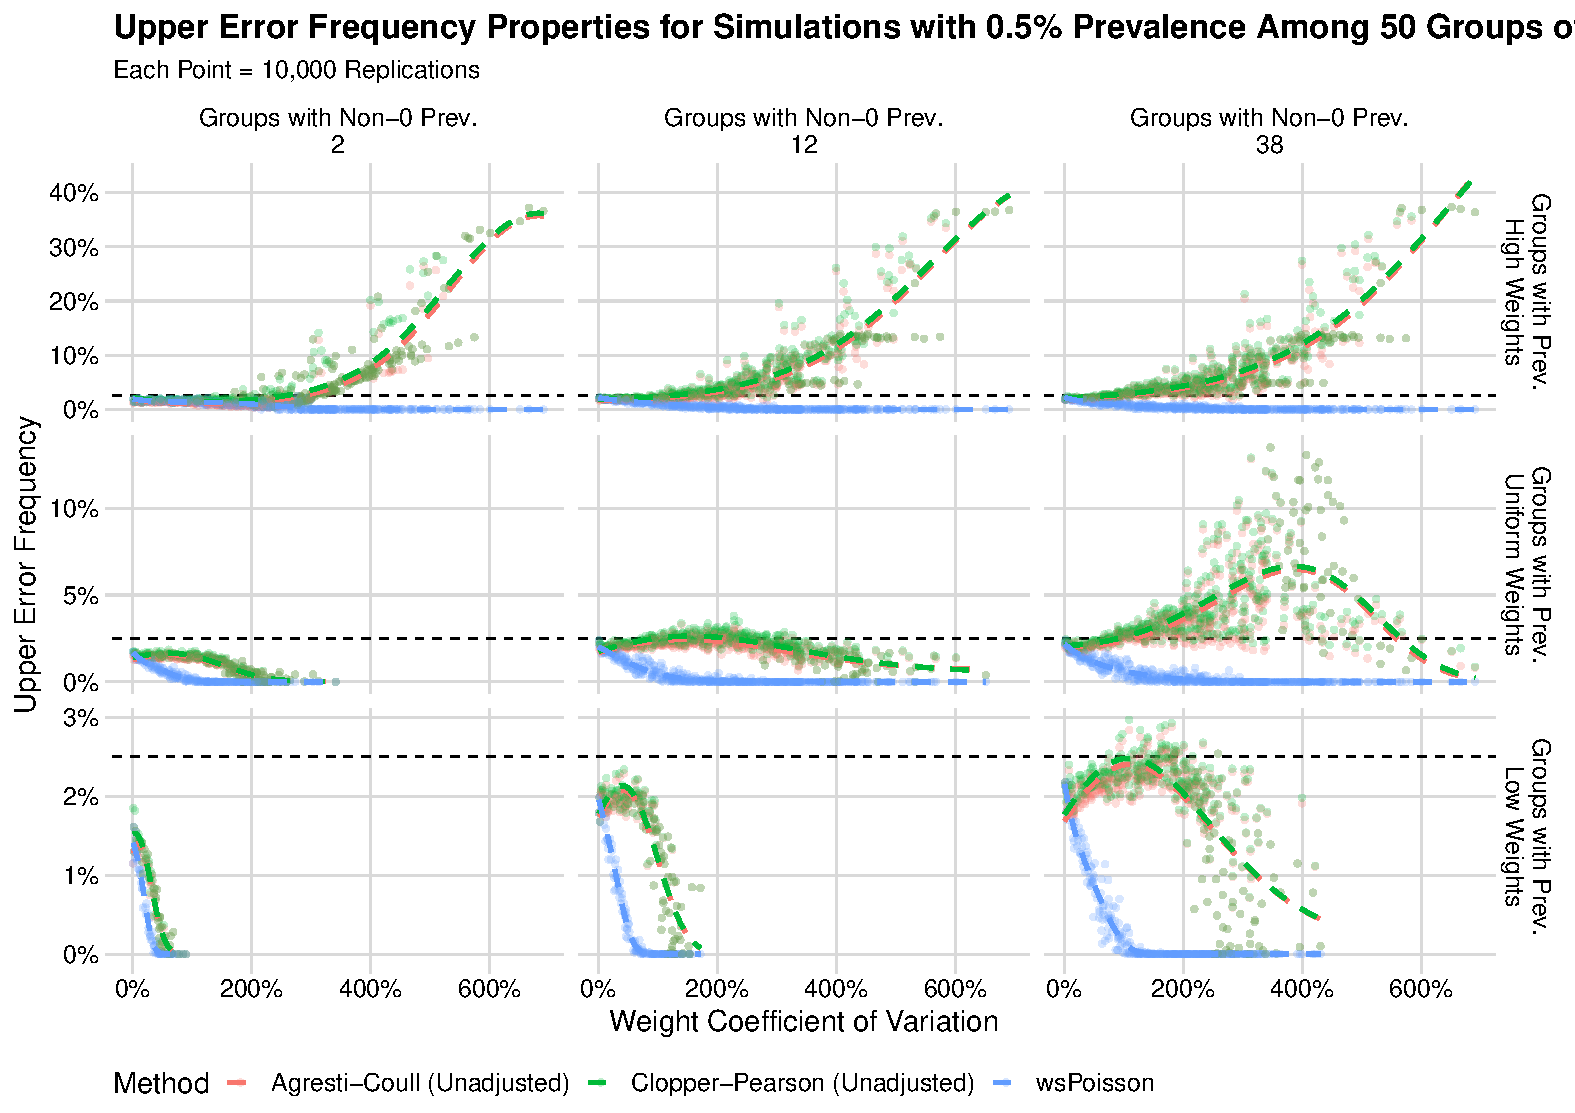
\includegraphics[width=\textwidth]{figures/perfect_upper_error_frequency_50_0_005_reduced.pdf}
    \caption{Caption}
    \label{fig:perfect_upper_error_frequency_50_0_005_reduced}
\end{figure}


\begin{figure}
    \centering
    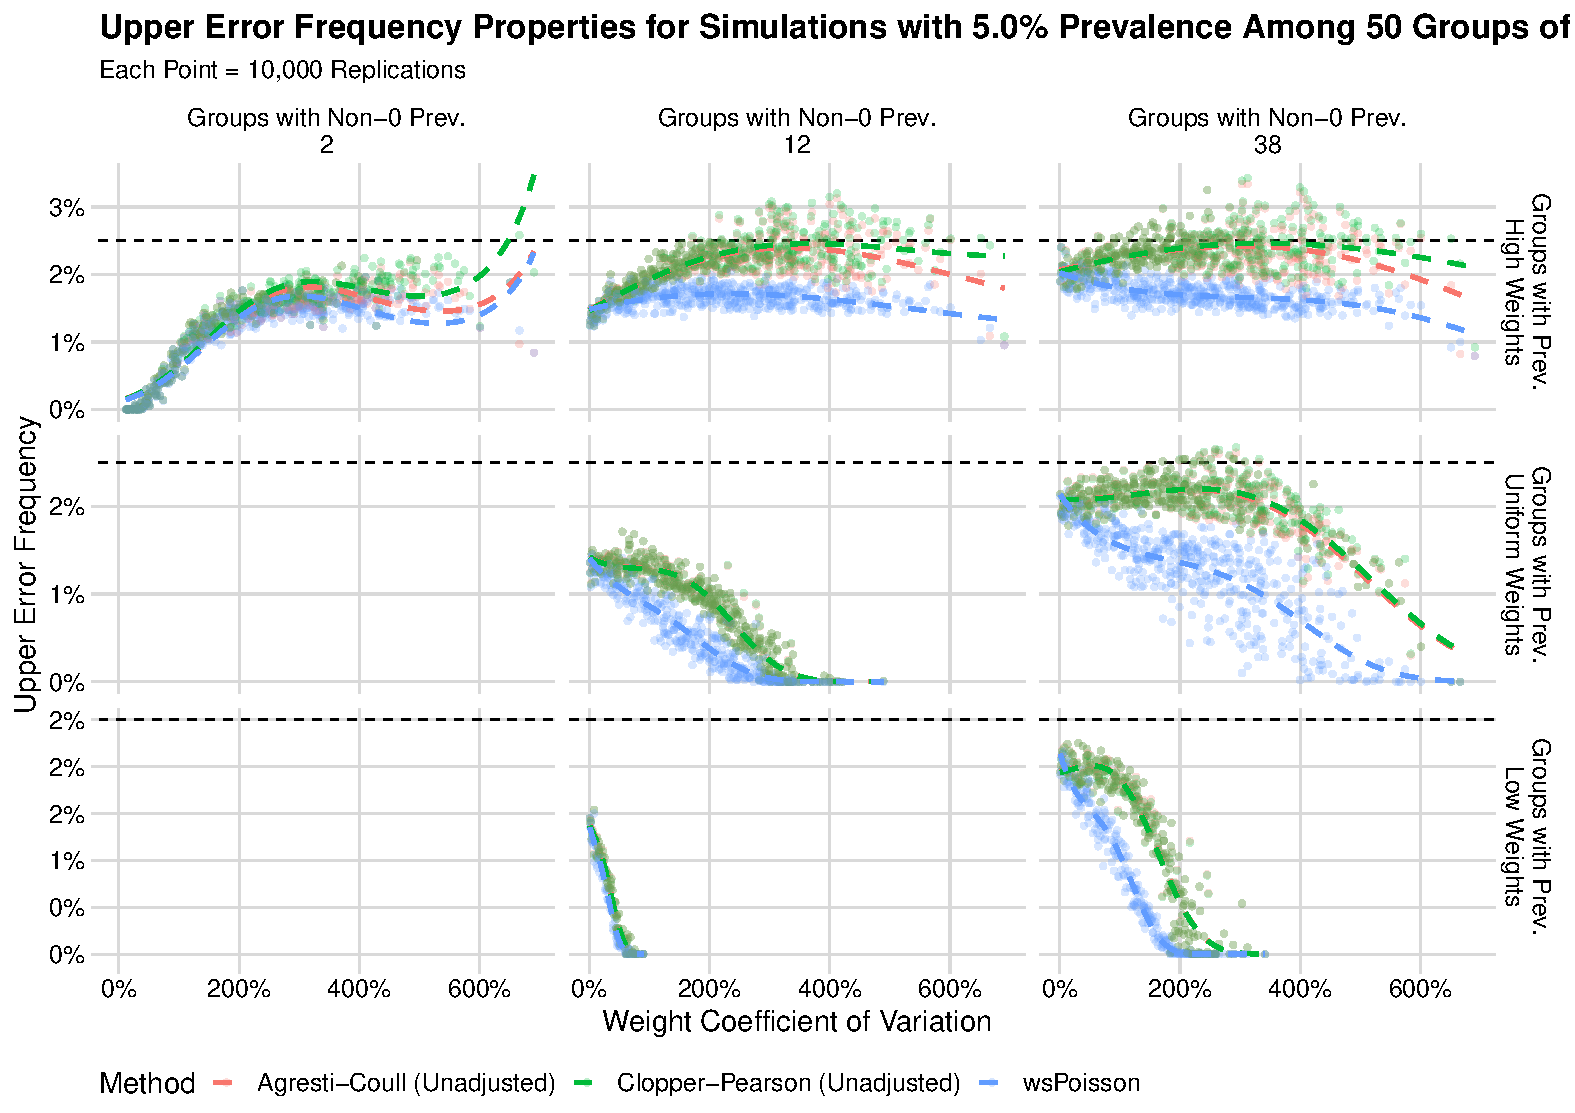
\includegraphics[width=\textwidth]{figures/perfect_upper_error_frequency_50_0_05_reduced.pdf}
    \caption{Caption}
    \label{fig:perfect_upper_error_frequency_50_0_05_reduced}
\end{figure}


\begin{figure}
    \centering
    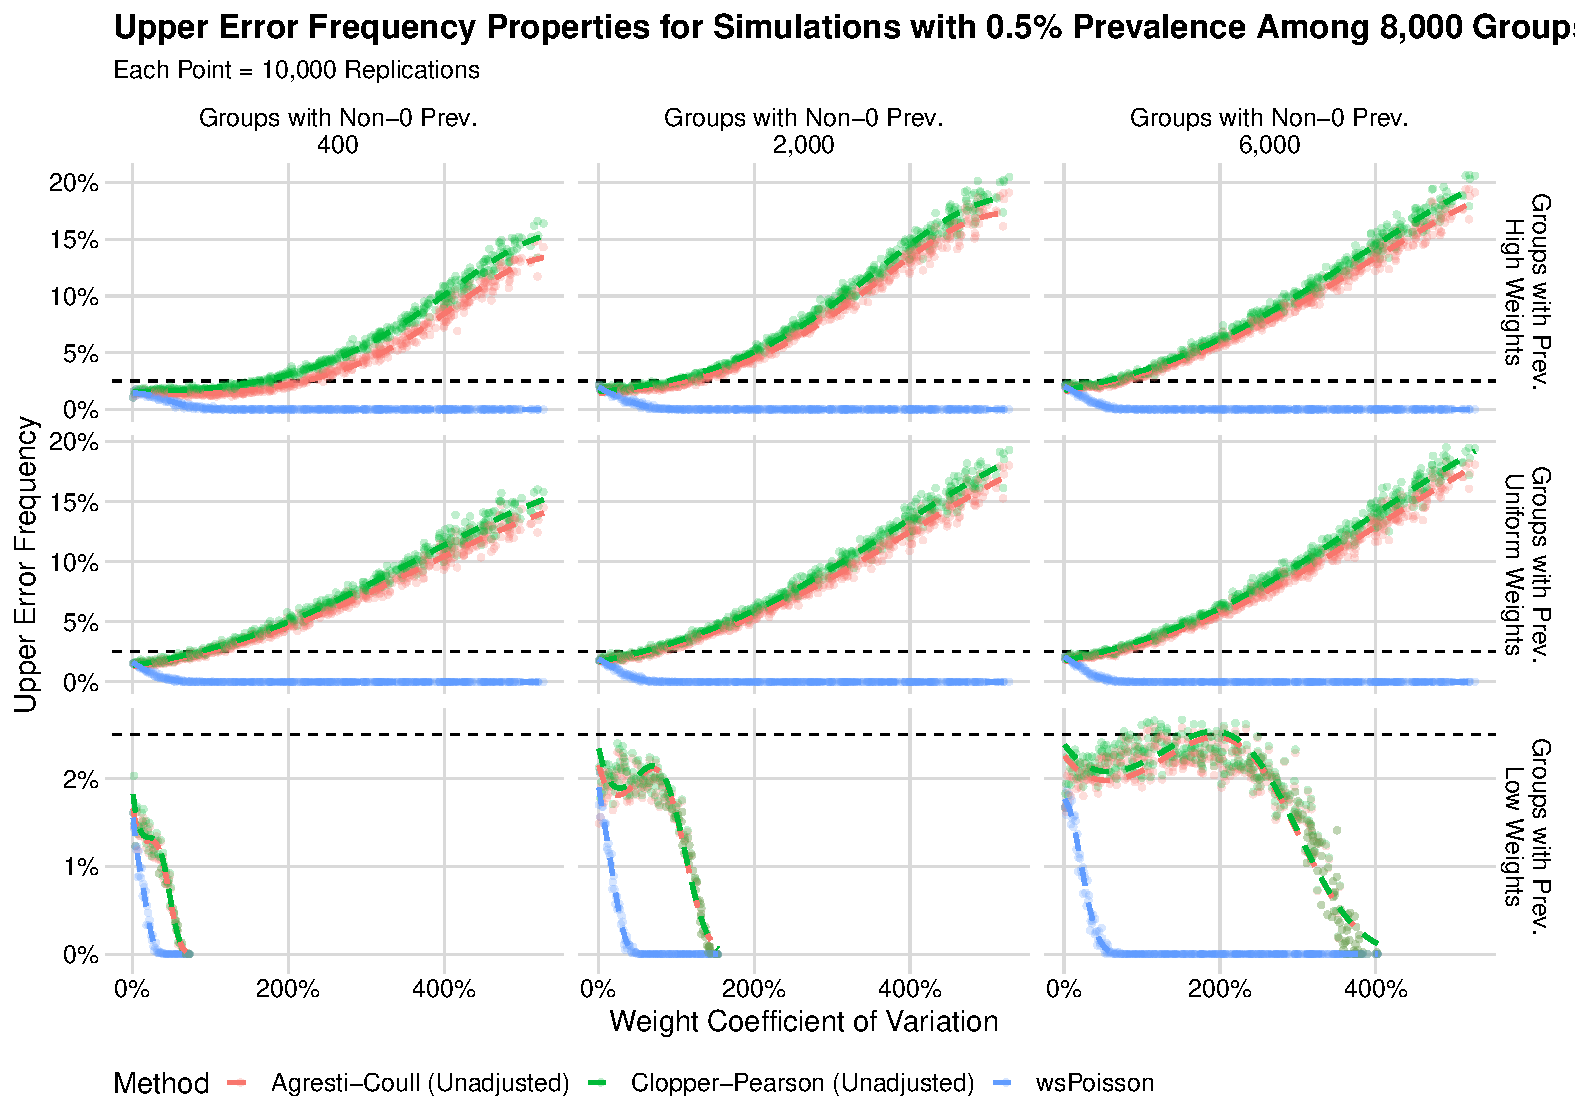
\includegraphics[width=\textwidth]{figures/perfect_upper_error_frequency_8000_0_005_reduced.pdf}
    \caption{Caption}
    \label{fig:perfect_upper_error_frequency_8000_0_005_reduced}
\end{figure}

\begin{figure}
    \centering
    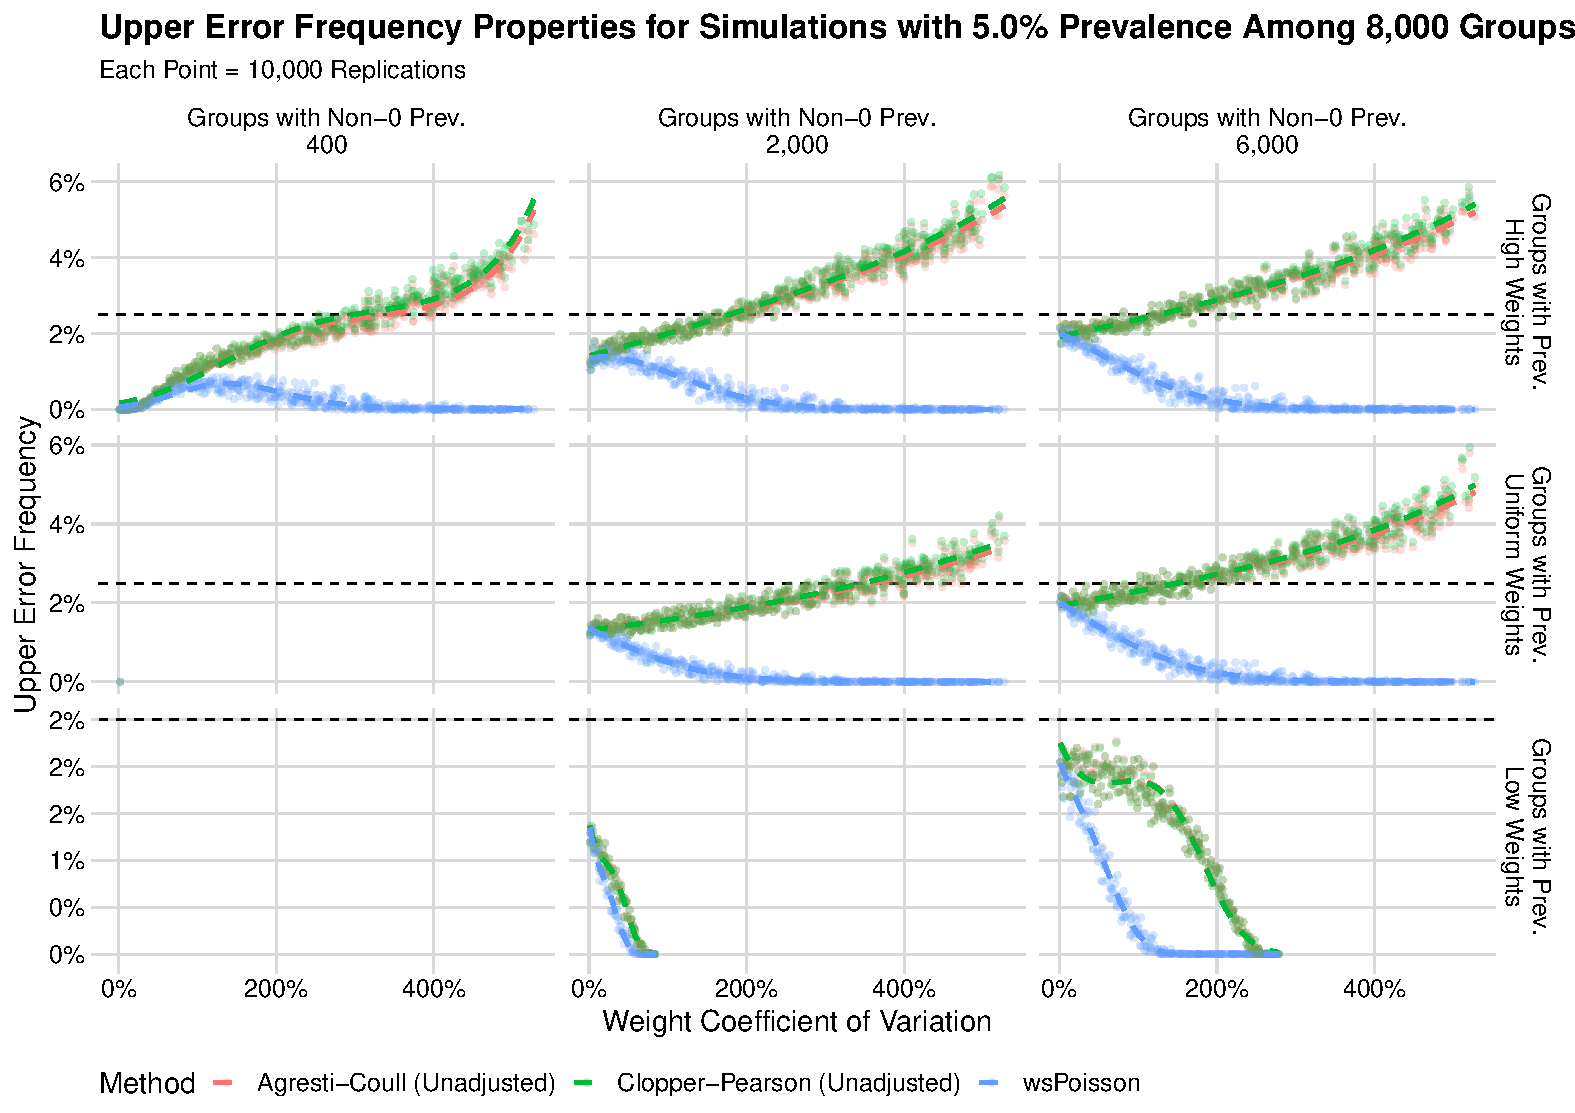
\includegraphics[width=\textwidth]{figures/perfect_upper_error_frequency_8000_0_05_reduced.pdf}
    \caption{Caption}
    \label{fig:perfect_upper_error_frequency_8000_0_05_reduced.pdf}
\end{figure}

\subsection{Estimating Prevalence from a Weighted Sample with an  Imperfect Assay}

\begin{figure}
    \centering
    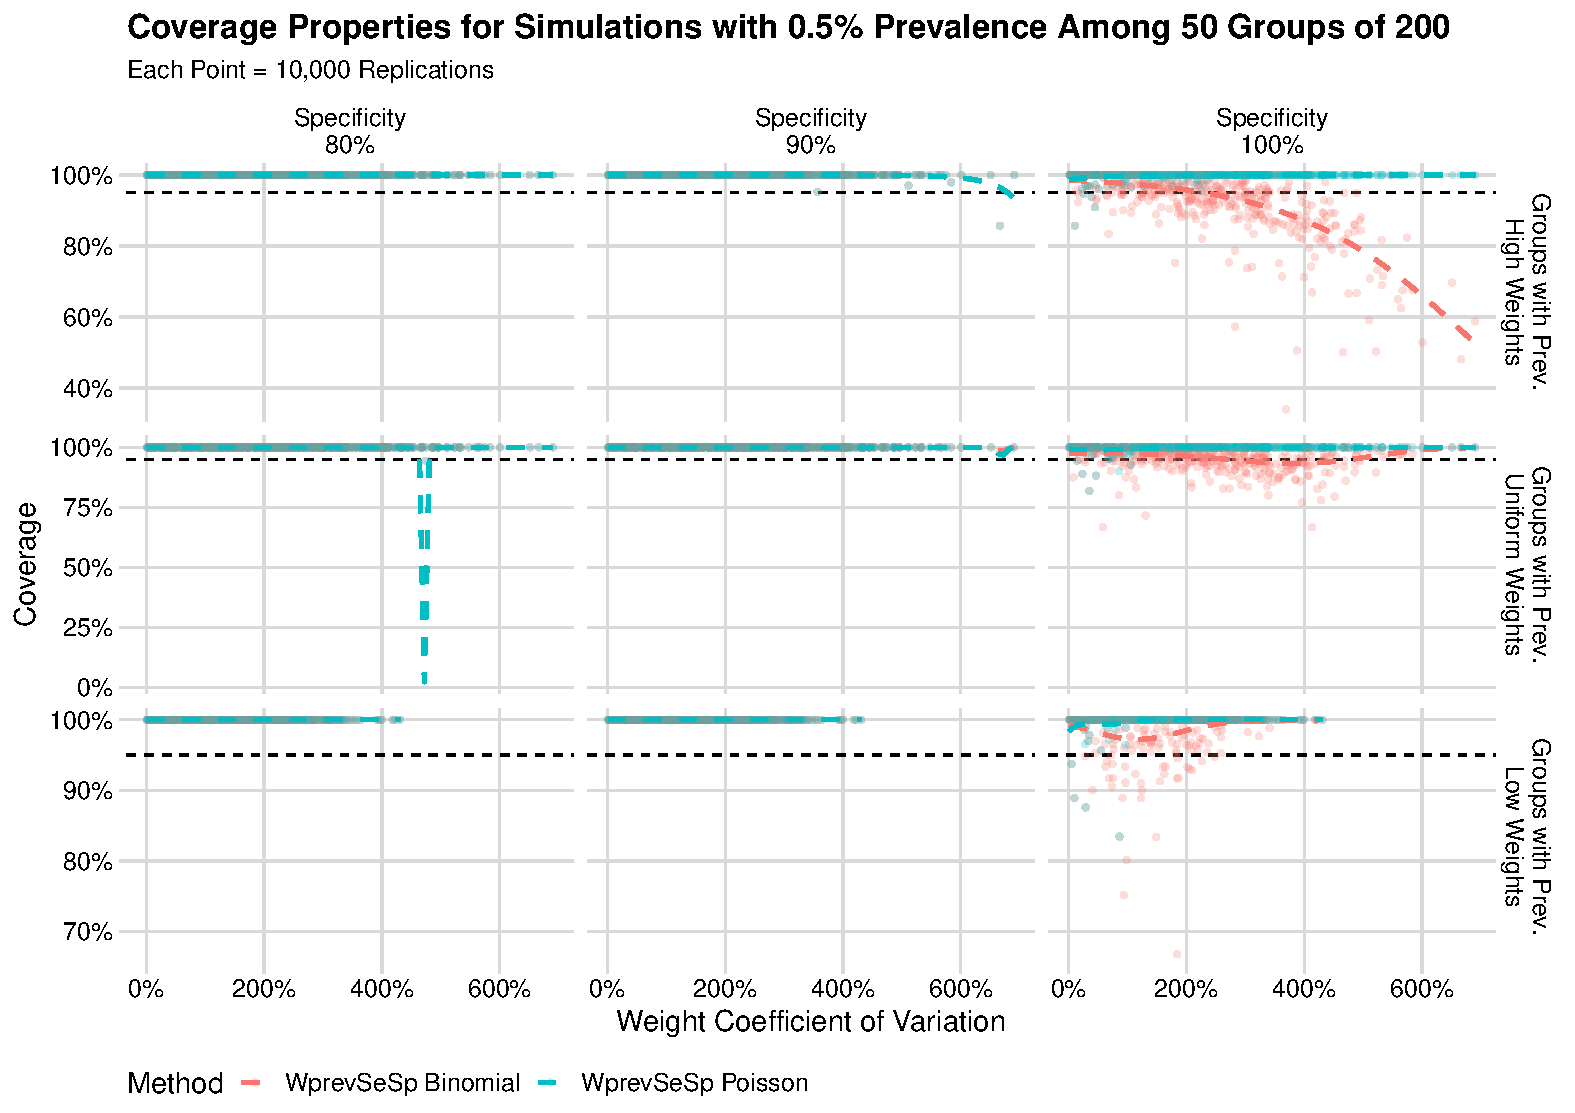
\includegraphics[width=\textwidth]{figures/imperfect_coverage_50_0_005_reduced.pdf}
    \caption{Caption}
    \label{fig:imperfect_coverage_50_0_005_reduced}
\end{figure}


\begin{figure}
    \centering
    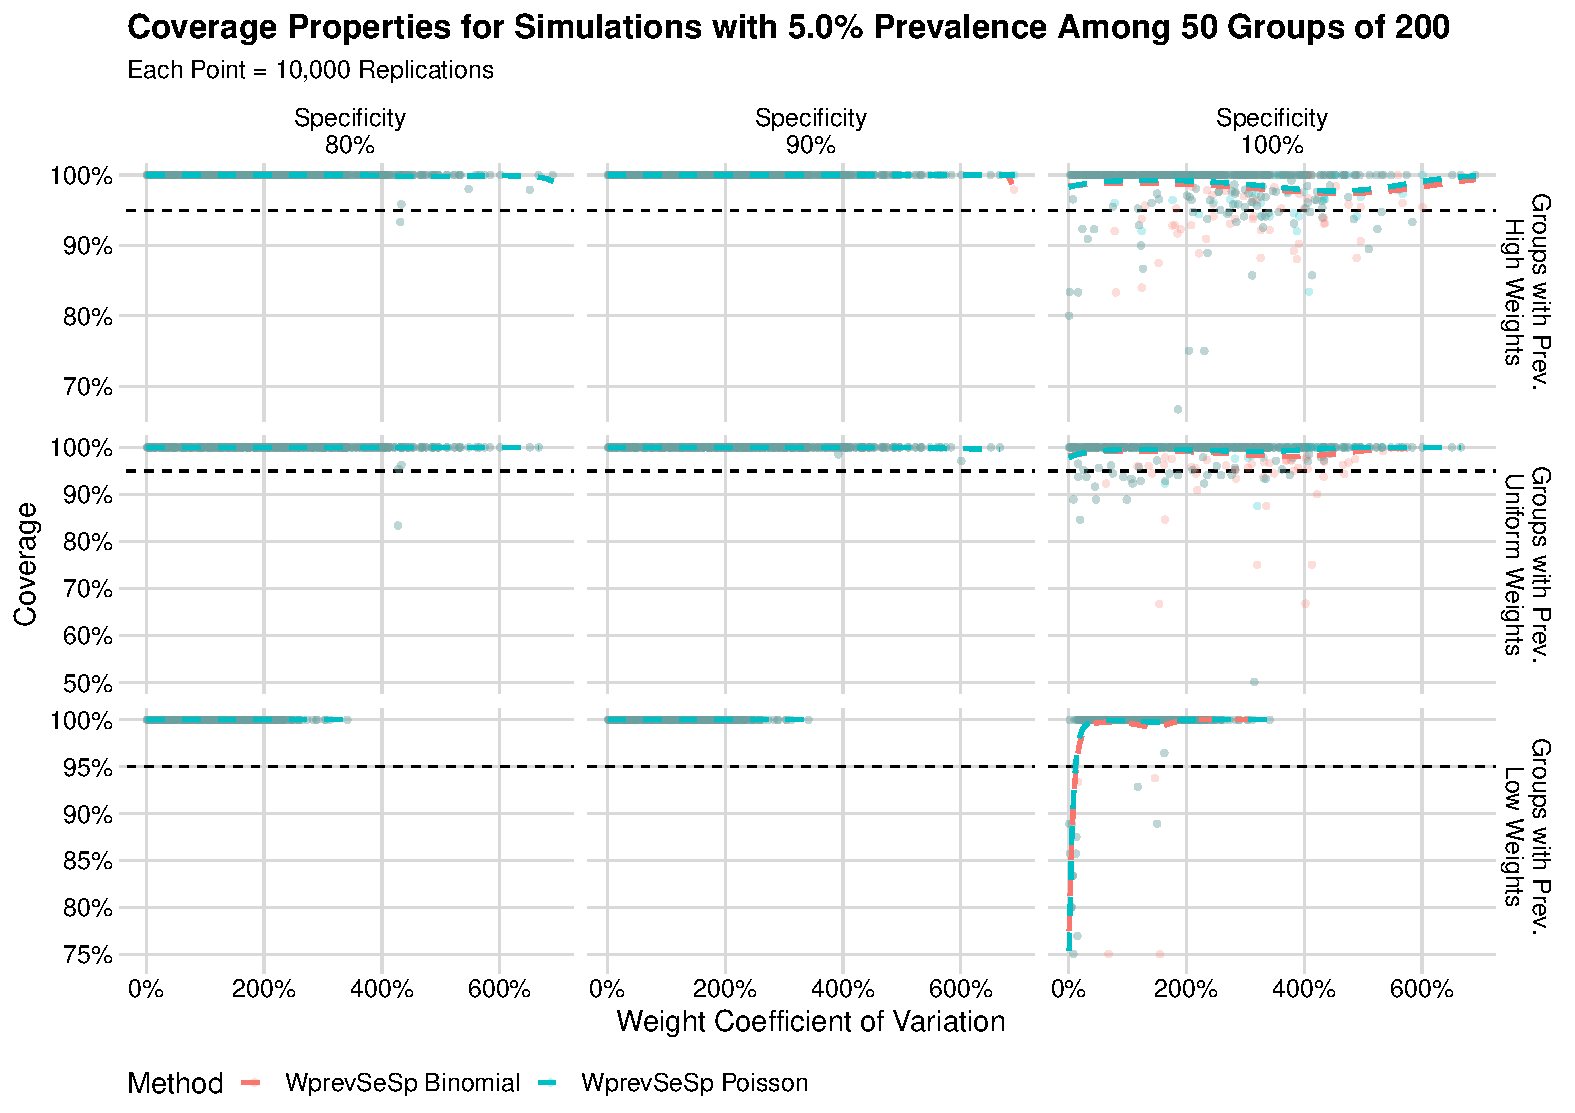
\includegraphics[width=\textwidth]{figures/imperfect_coverage_50_0_05_reduced.pdf}
    \caption{Caption}
    \label{fig:imperfect_coverage_50_0_05_reduced}
\end{figure}


\begin{figure}
    \centering
    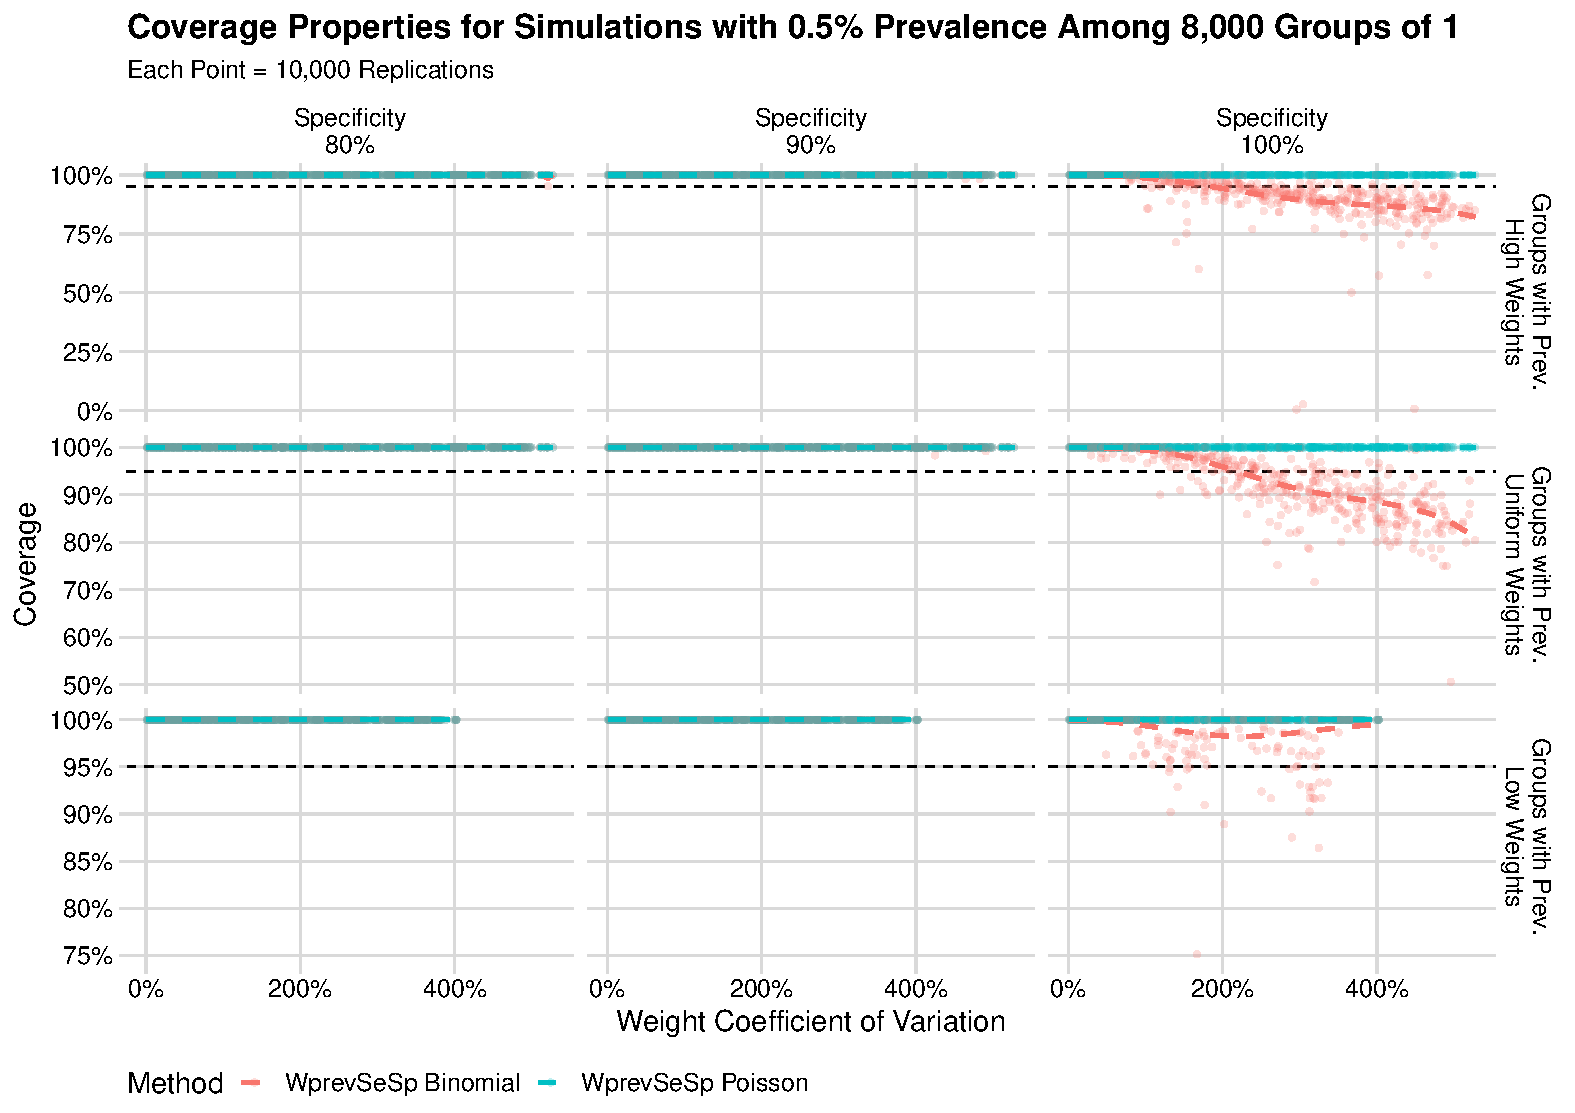
\includegraphics[width=\textwidth]{figures/imperfect_coverage_8000_0_005_reduced.pdf}
    \caption{Caption}
    \label{fig:imperfect_coverage_8000_0_005_reduced}
\end{figure}

\begin{figure}
    \centering
    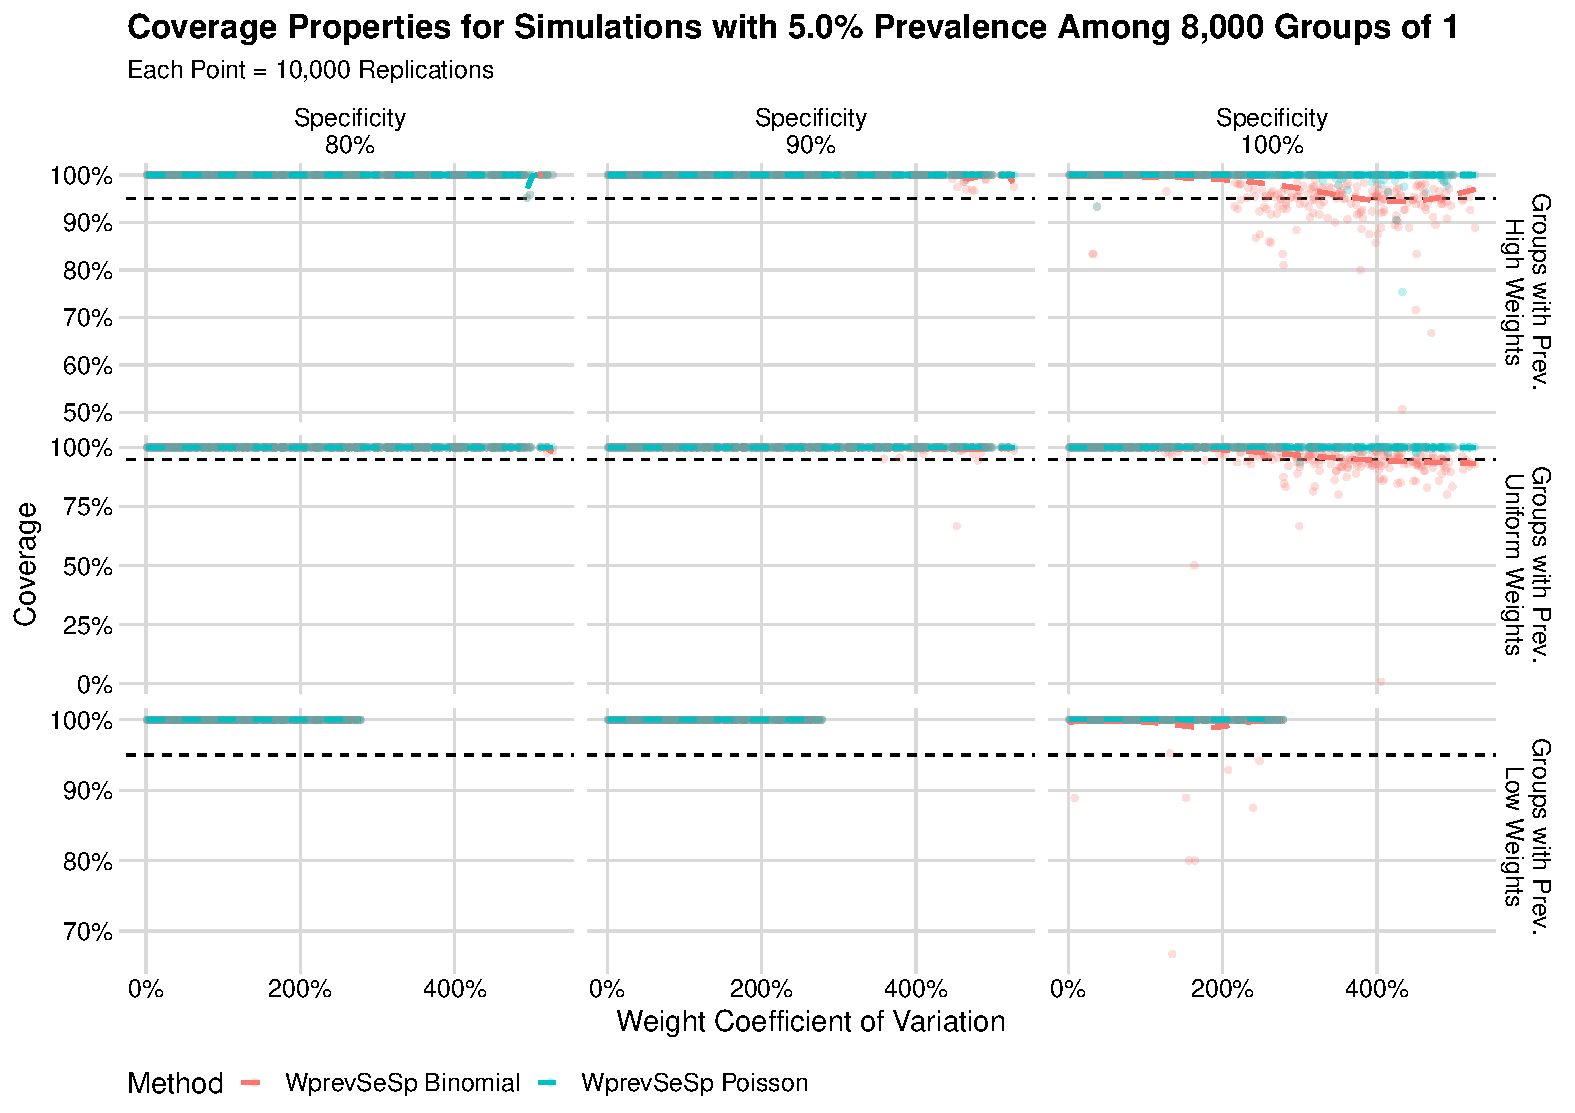
\includegraphics[width=\textwidth]{figures/imperfect_coverage_8000_0_05_reduced.pdf}
    \caption{Caption}
    \label{fig:imperfect_coverage_8000_0_05_reduced.pdf}
\end{figure}


\begin{figure}
    \centering
    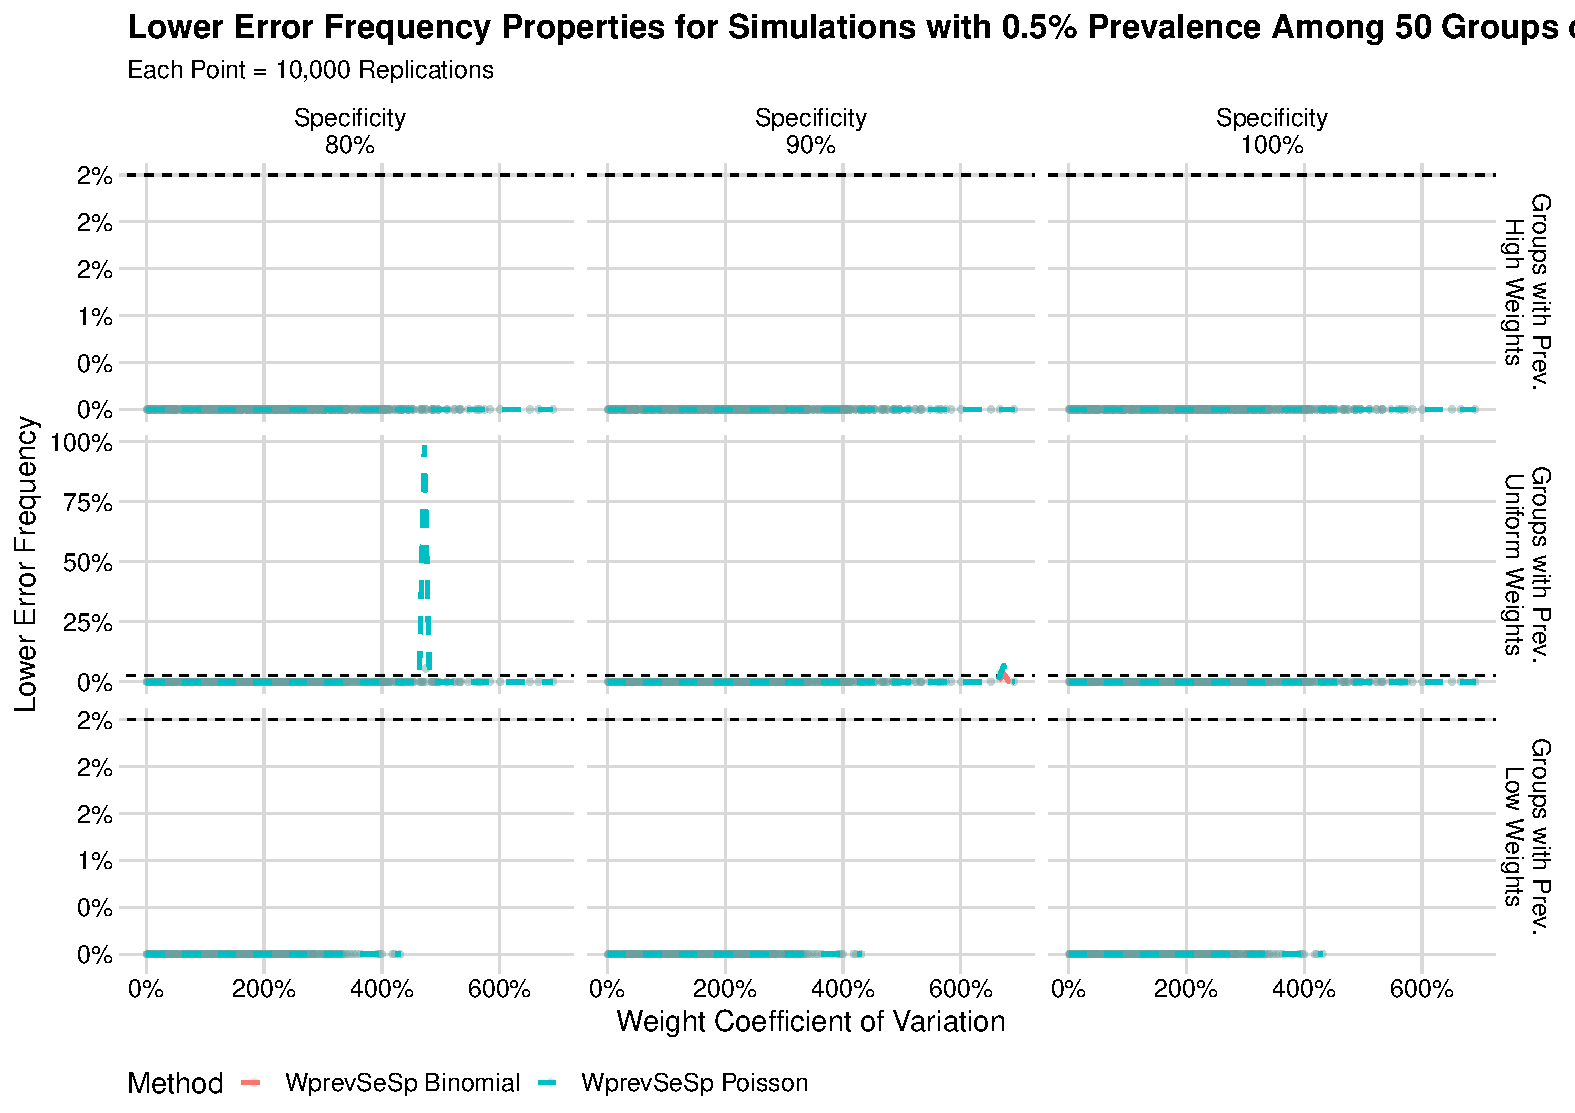
\includegraphics[width=\textwidth]{figures/imperfect_lower_error_frequency_50_0_005_reduced.pdf}
    \caption{Caption}
    \label{fig:imperfect_lower_error_frequency_50_0_005_reduced}
\end{figure}


\begin{figure}
    \centering
    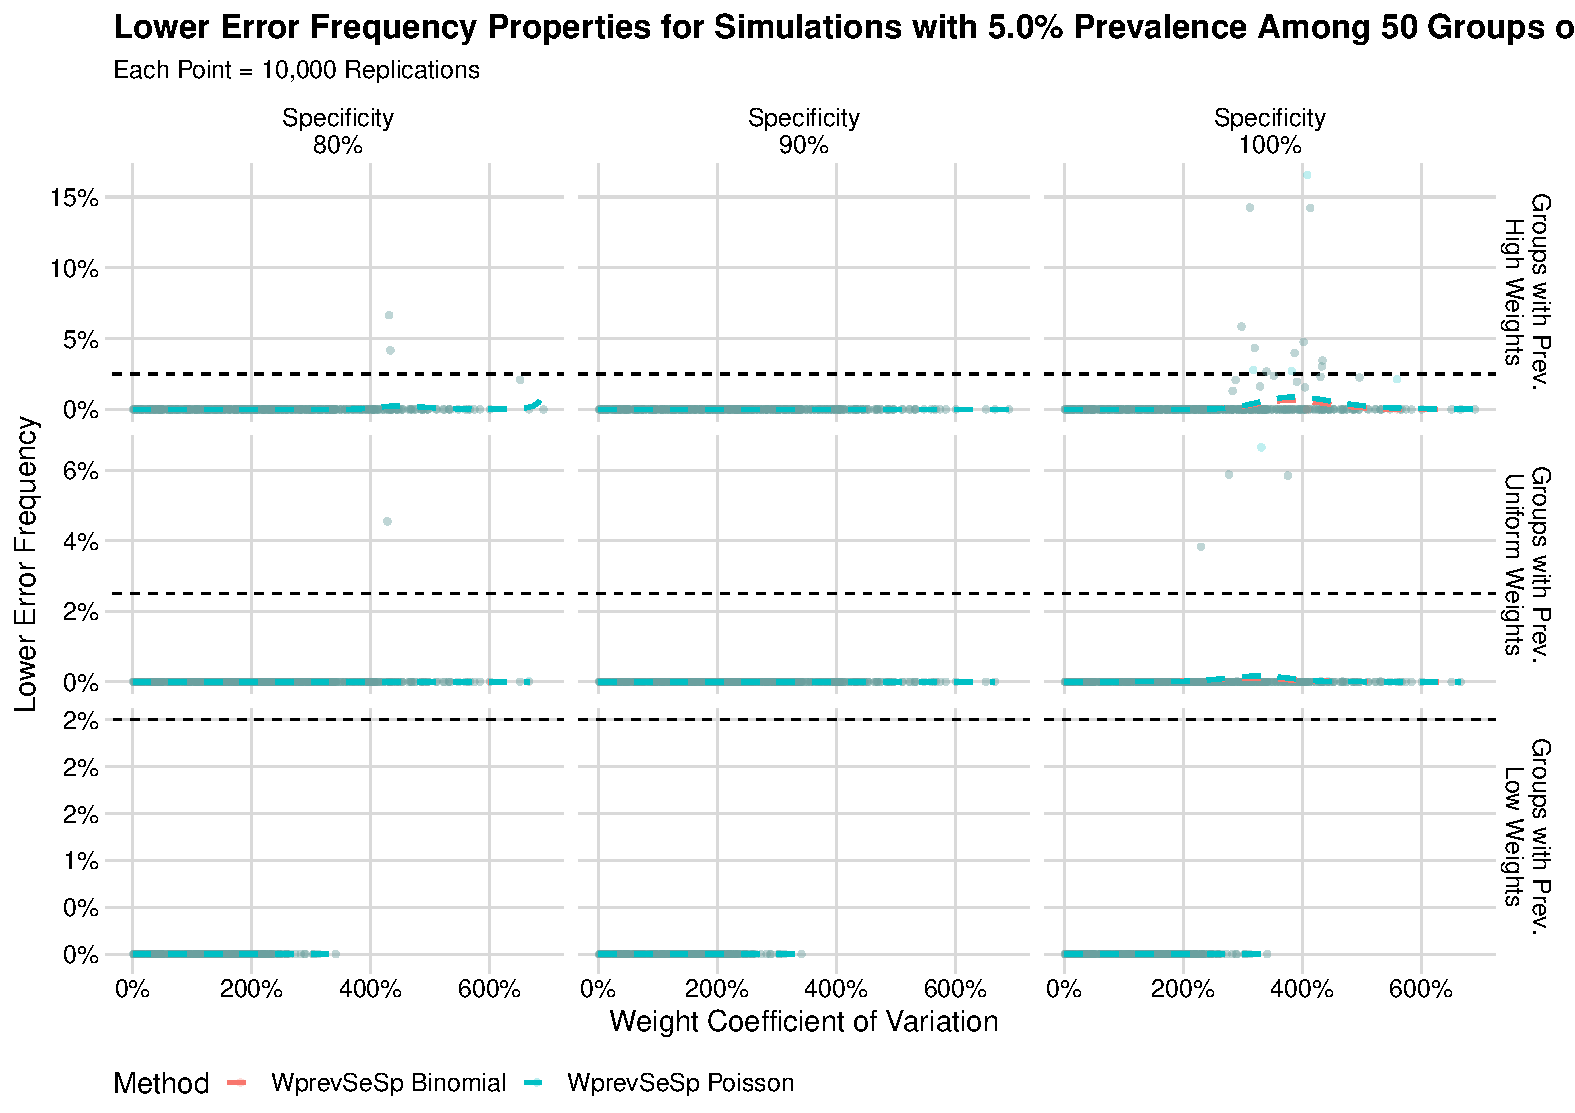
\includegraphics[width=\textwidth]{figures/imperfect_lower_error_frequency_50_0_05_reduced.pdf}
    \caption{Caption}
    \label{fig:imperfect_lower_error_frequency_50_0_05_reduced}
\end{figure}


\begin{figure}
    \centering
    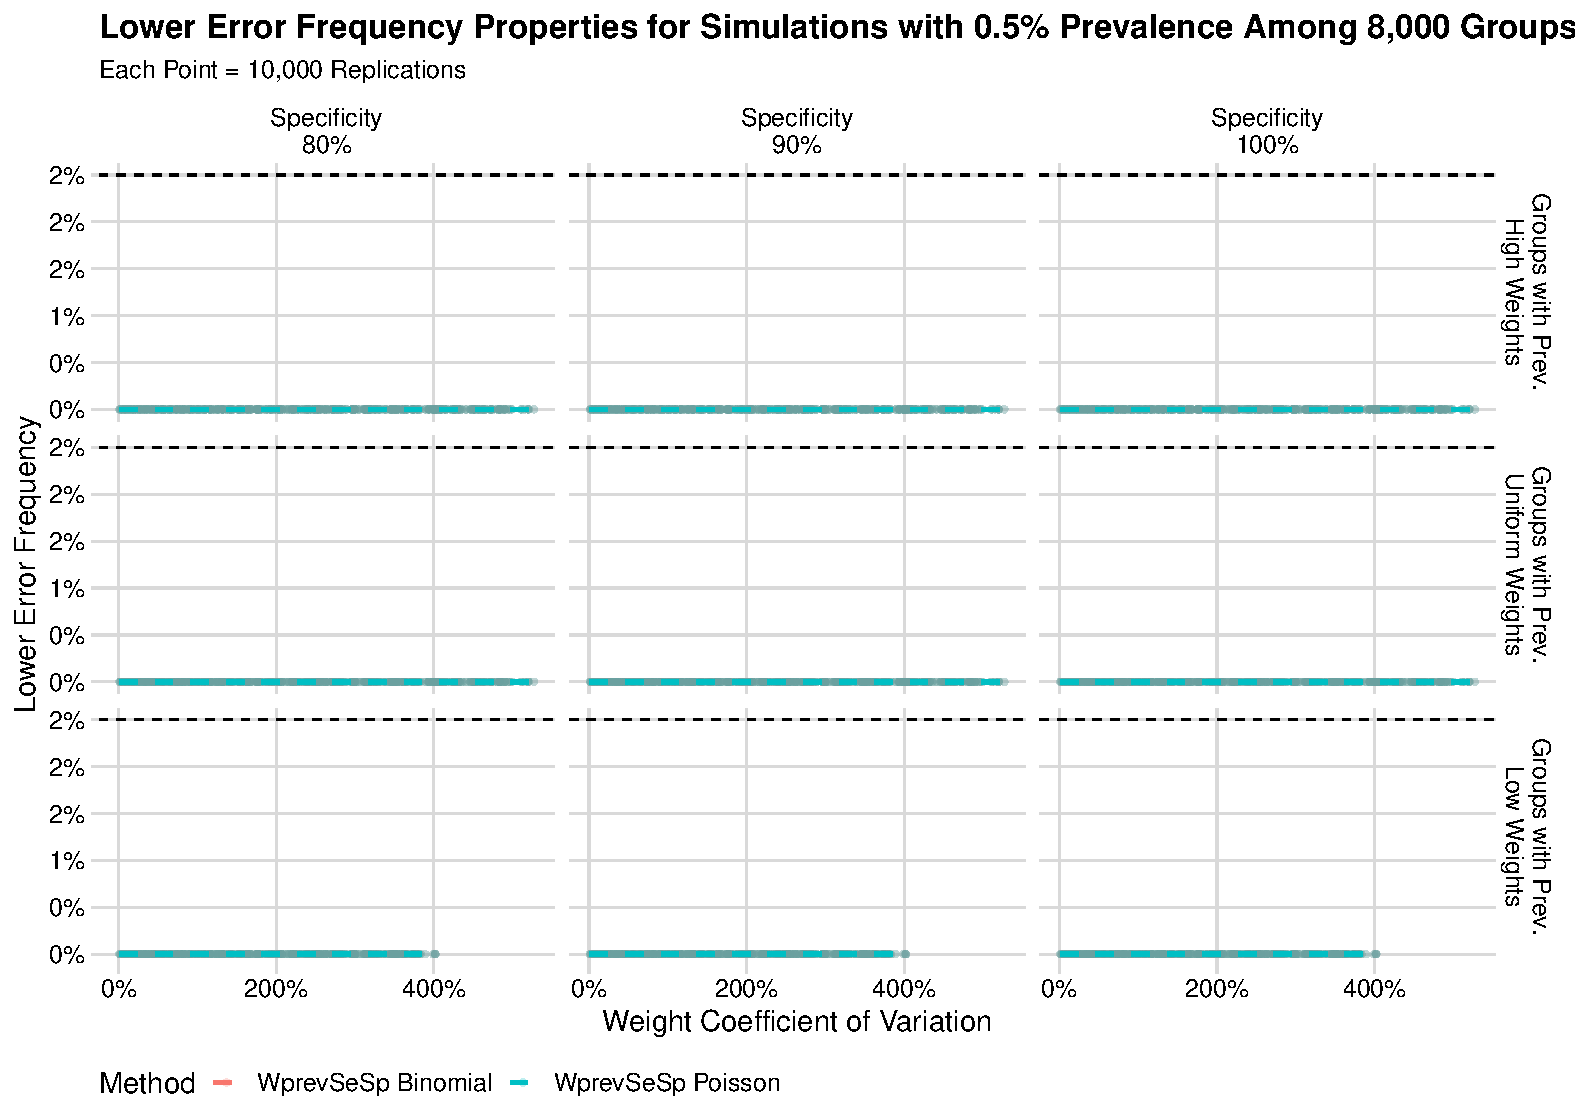
\includegraphics[width=\textwidth]{figures/imperfect_lower_error_frequency_8000_0_005_reduced.pdf}
    \caption{Caption}
    \label{fig:imperfect_lower_error_frequency_8000_0_005_reduced}
\end{figure}

\begin{figure}
    \centering
    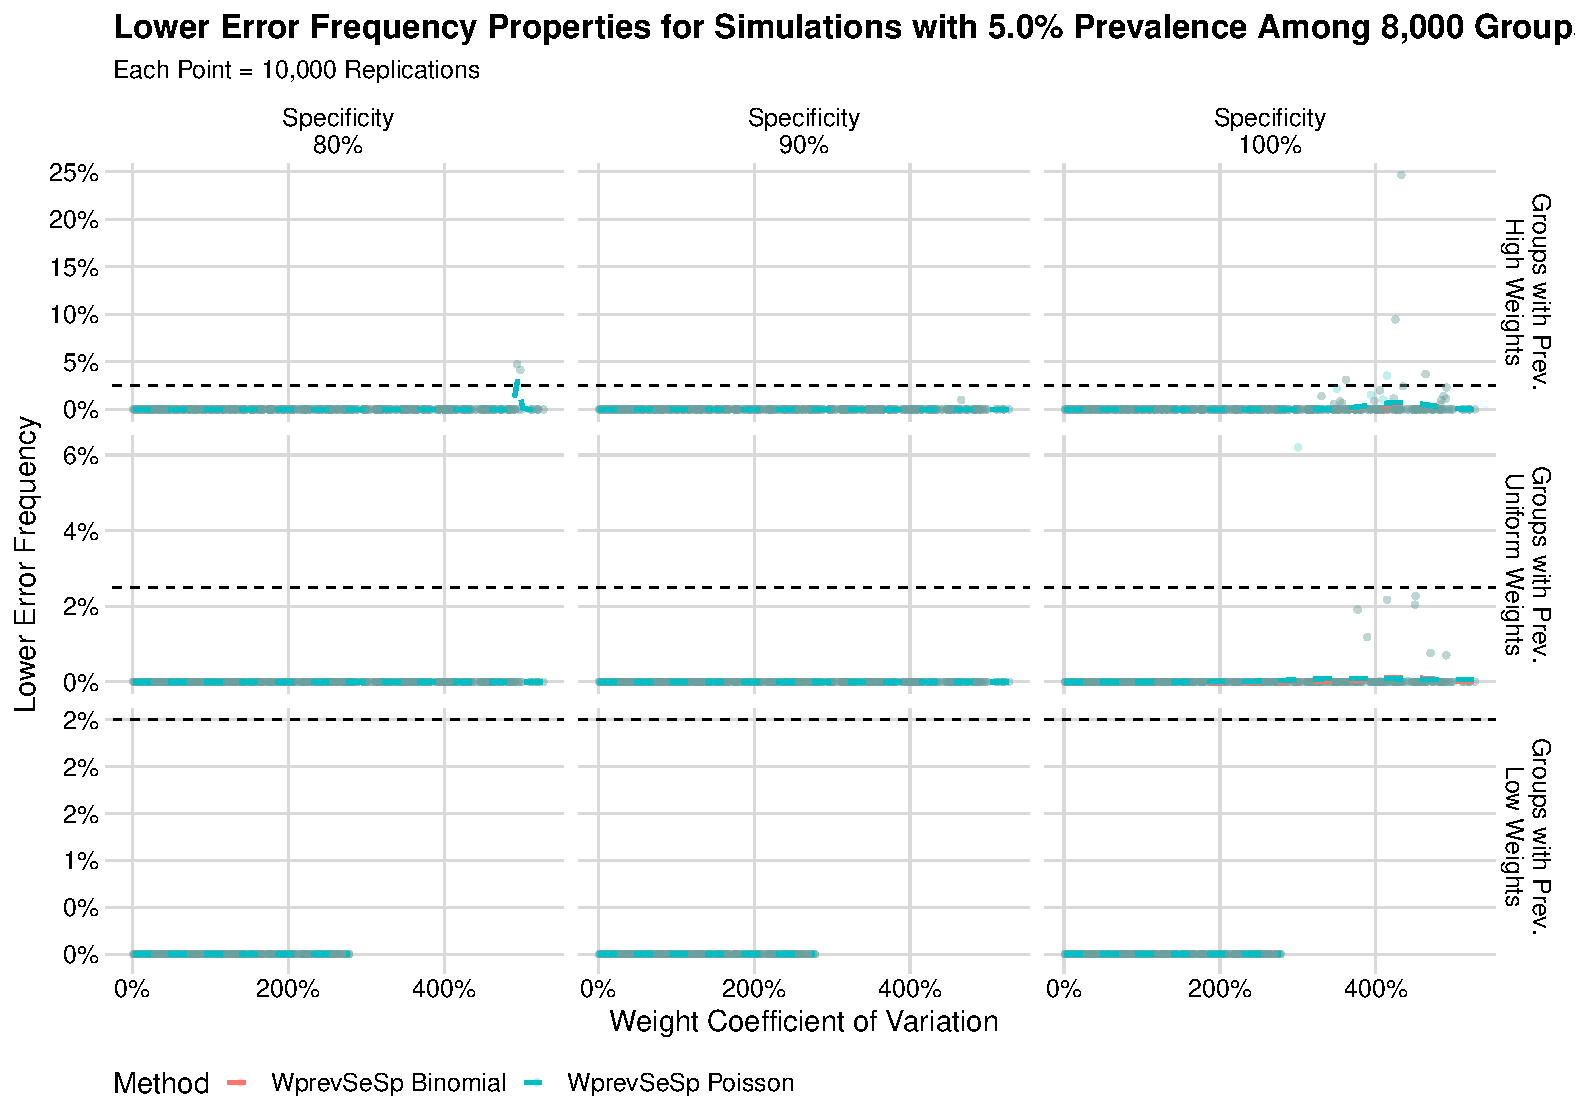
\includegraphics[width=\textwidth]{figures/imperfect_lower_error_frequency_8000_0_05_reduced.pdf}
    \caption{Caption}
    \label{fig:imperfect_lower_error_frequency_8000_0_05_reduced.pdf}
\end{figure}

\begin{figure}
    \centering
    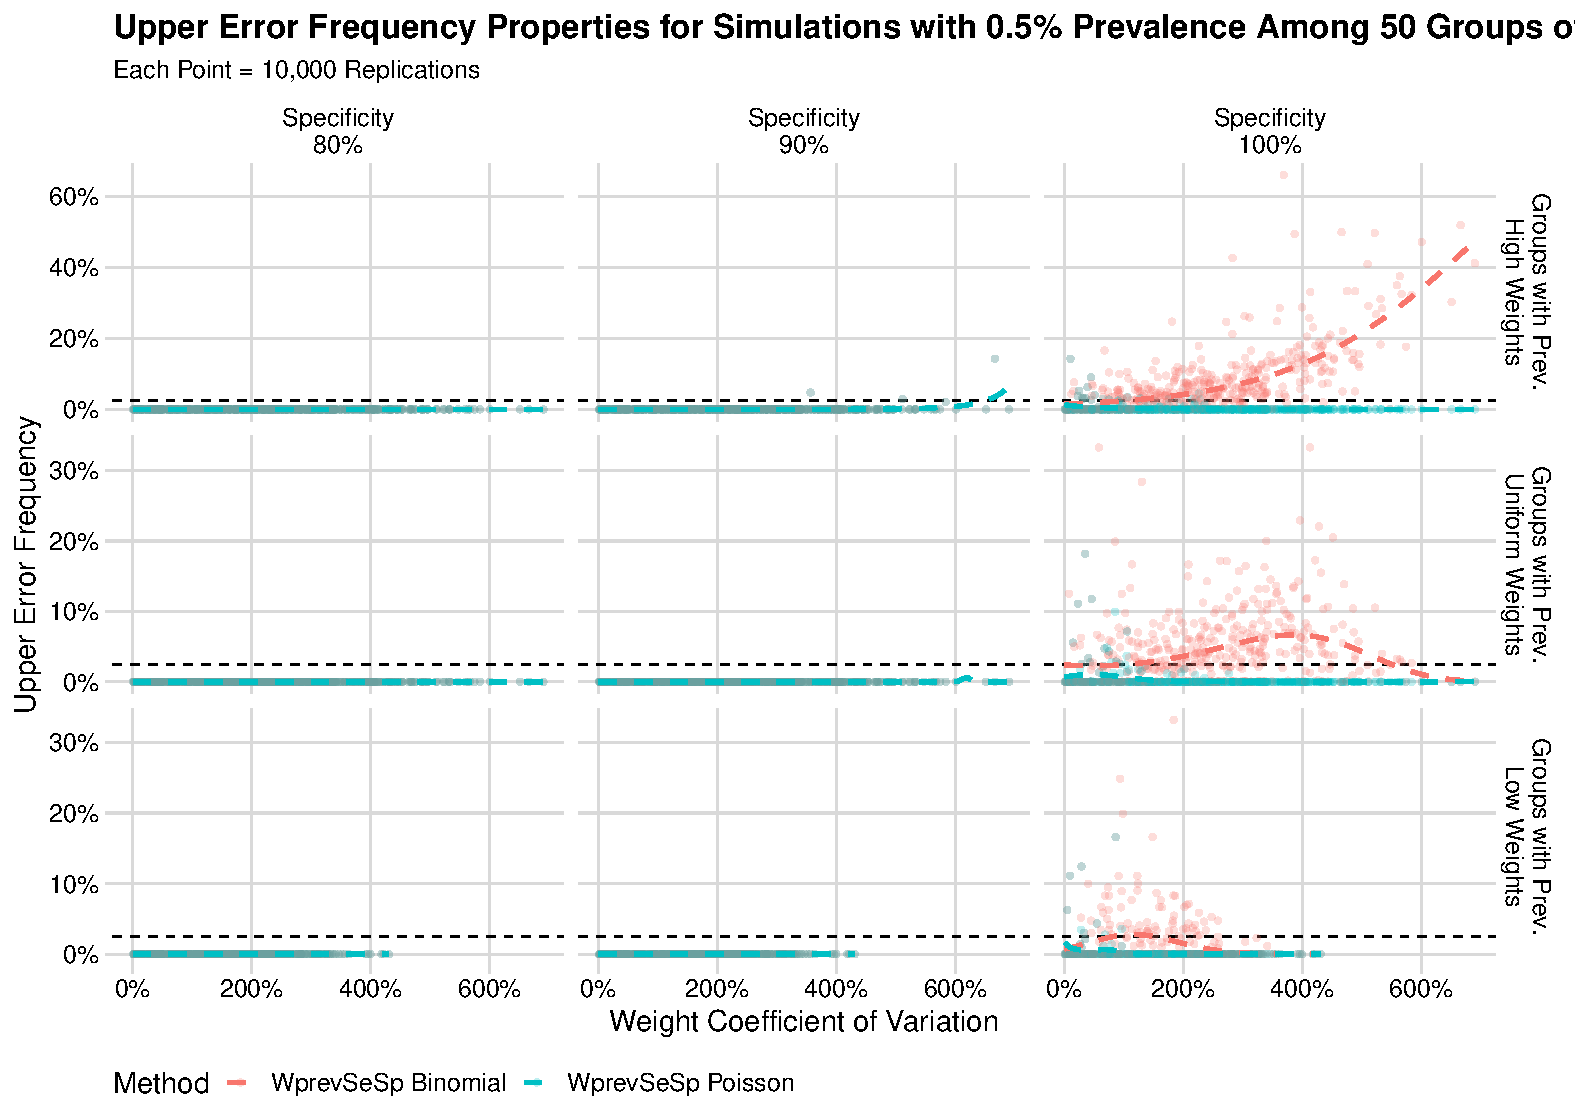
\includegraphics[width=\textwidth]{figures/imperfect_upper_error_frequency_50_0_005_reduced.pdf}
    \caption{Caption}
    \label{fig:imperfect_upper_error_frequency_50_0_005_reduced}
\end{figure}


\begin{figure}
    \centering
    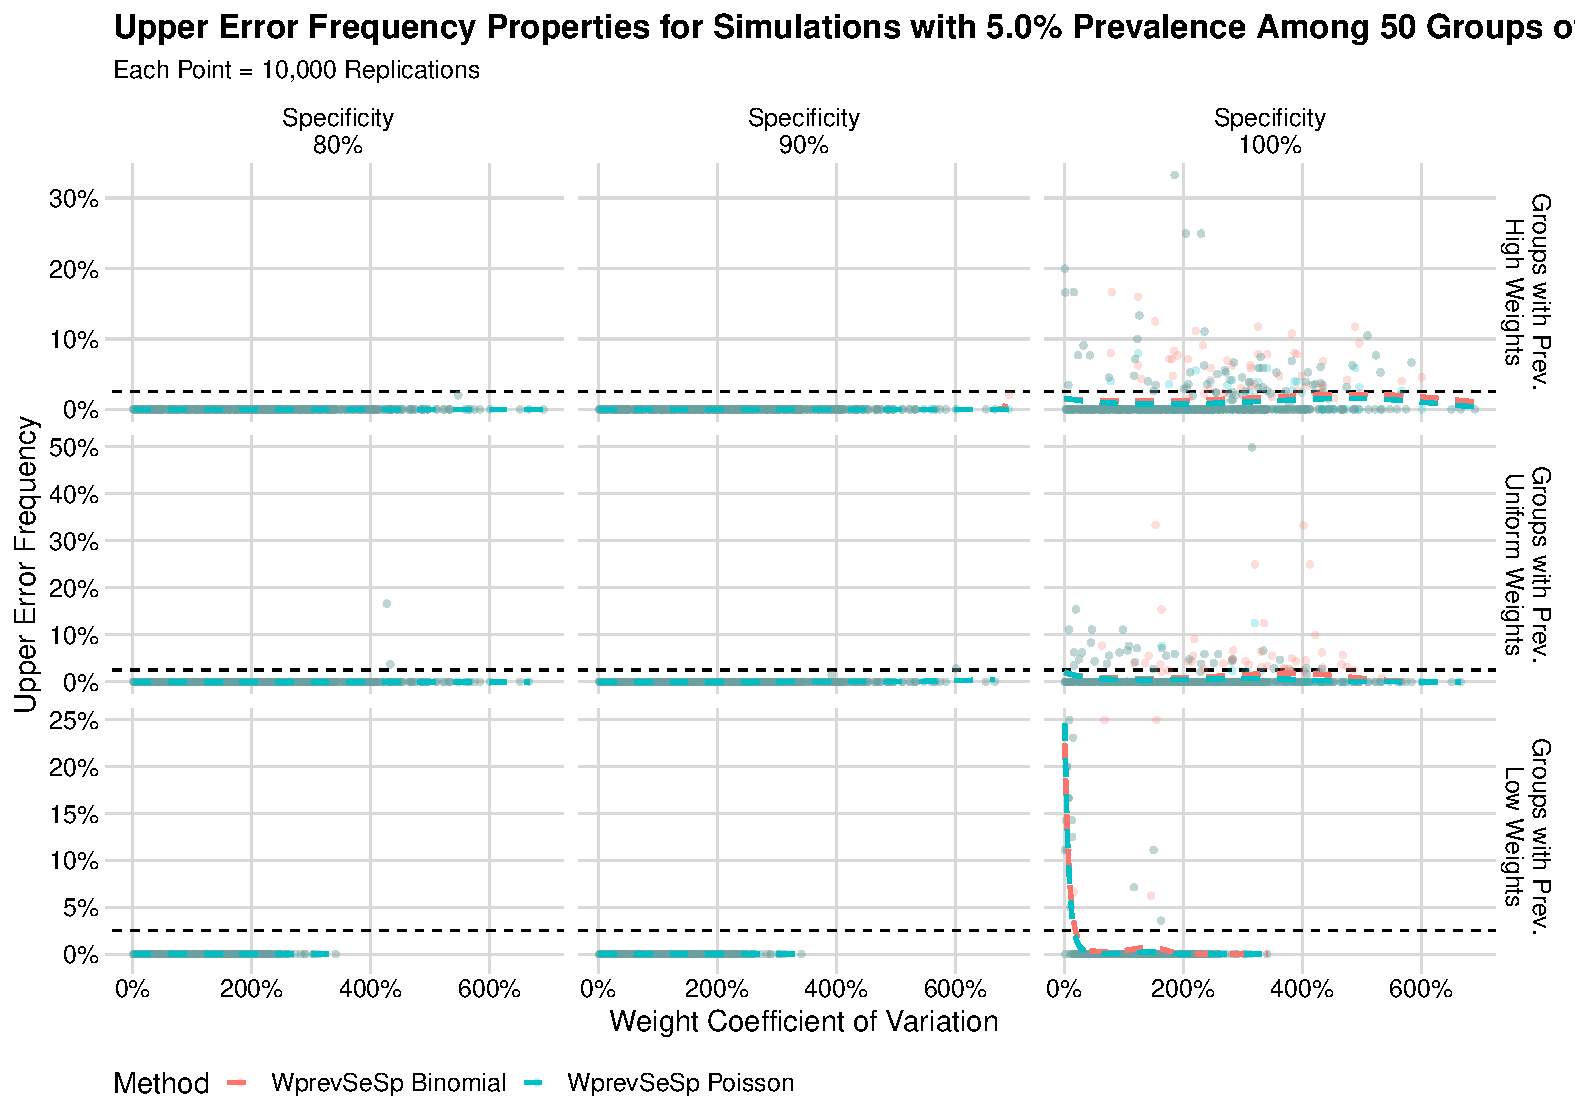
\includegraphics[width=\textwidth]{figures/imperfect_upper_error_frequency_50_0_05_reduced.pdf}
    \caption{Caption}
    \label{fig:imperfect_upper_error_frequency_50_0_05_reduced}
\end{figure}


\begin{figure}
    \centering
    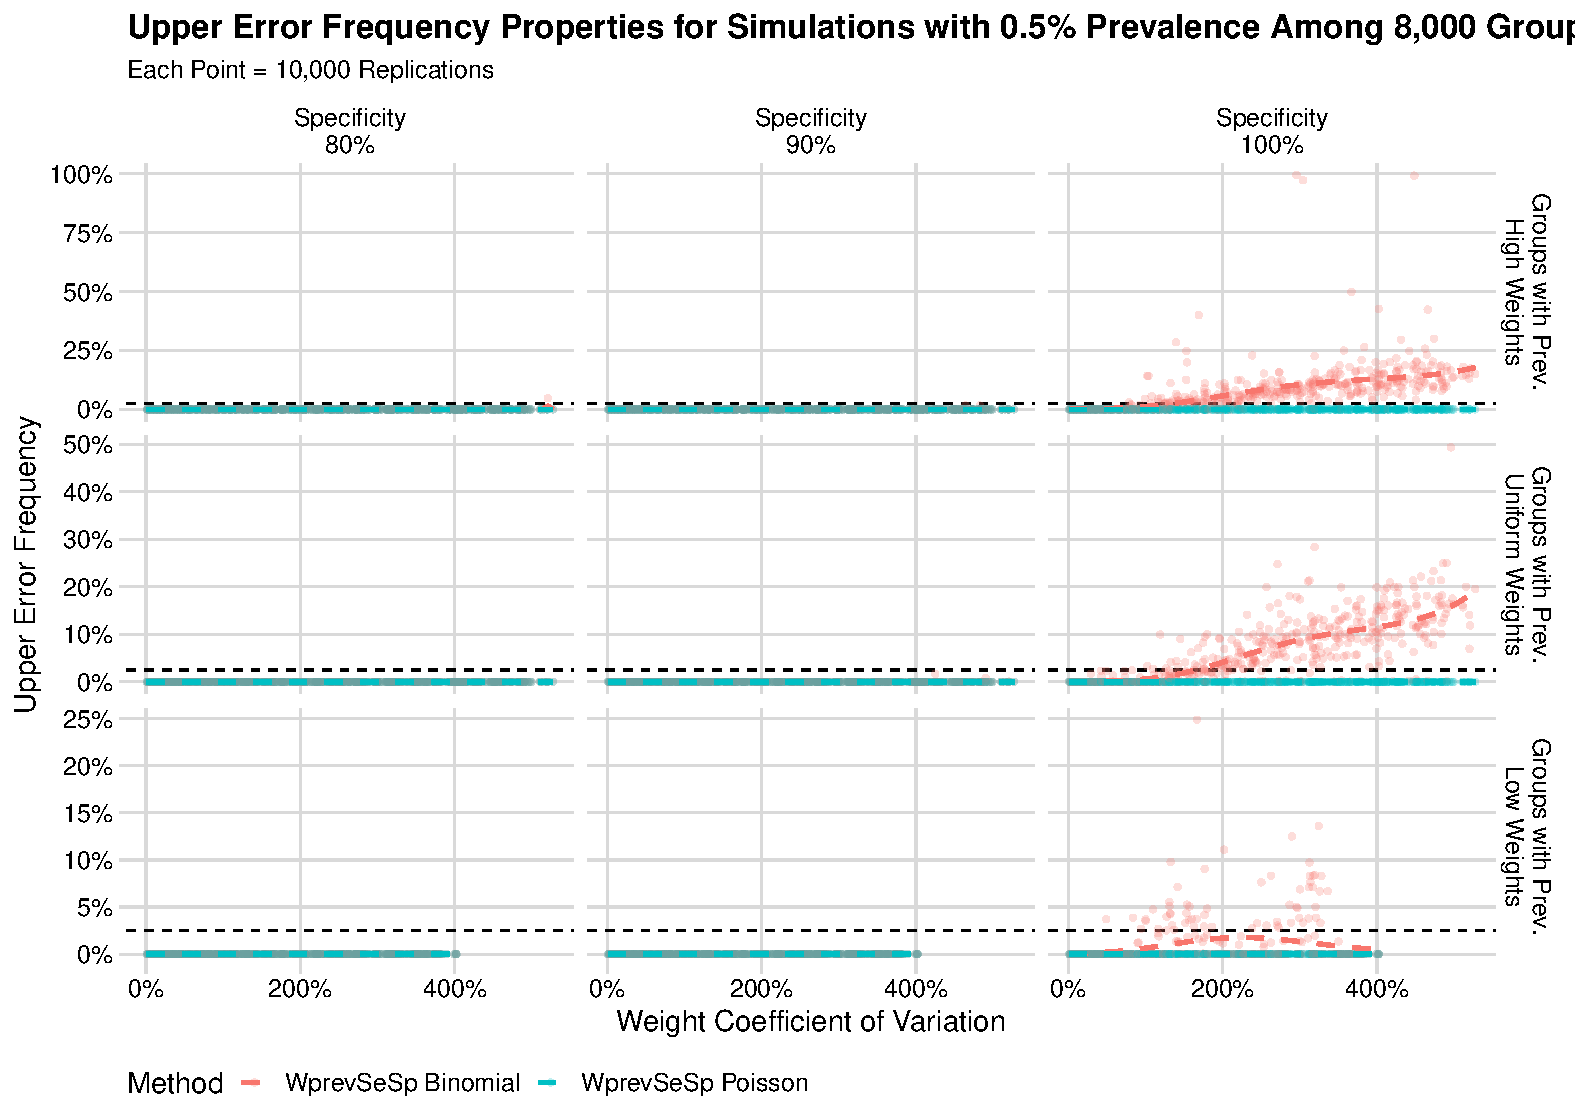
\includegraphics[width=\textwidth]{figures/imperfect_upper_error_frequency_8000_0_005_reduced.pdf}
    \caption{Caption}
    \label{fig:imperfect_upper_error_frequency_8000_0_005_reduced}
\end{figure}

\begin{figure}
    \centering
    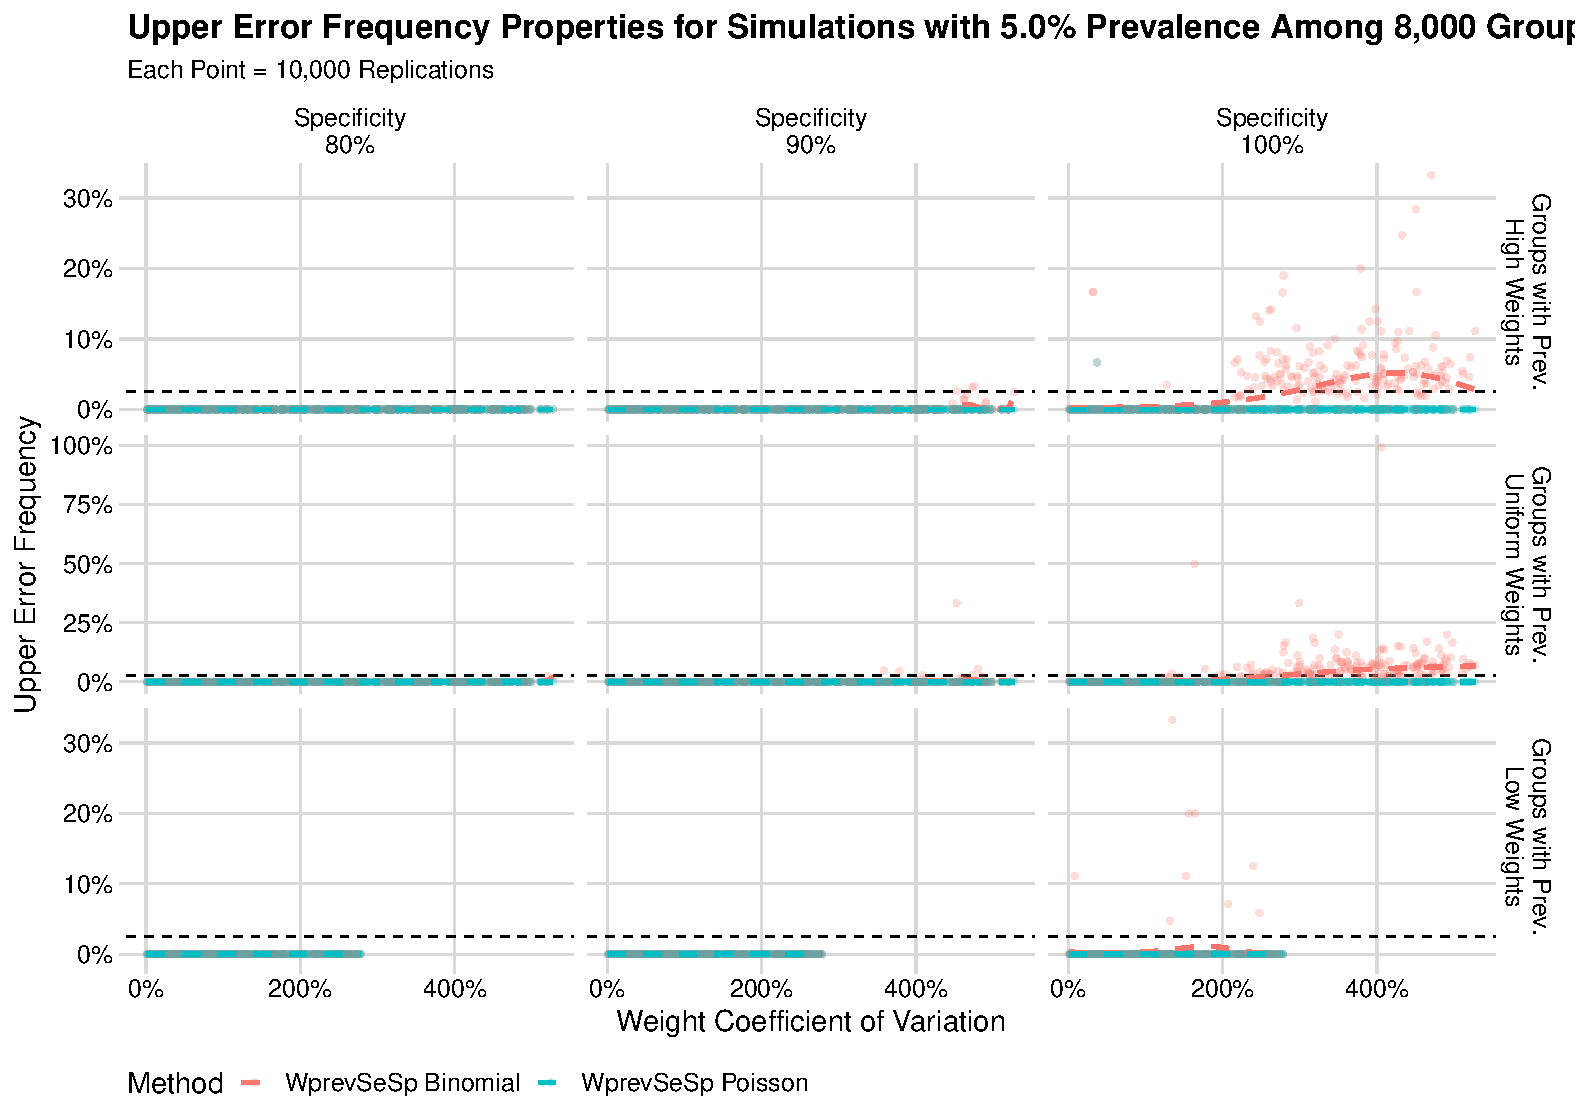
\includegraphics[width=\textwidth]{figures/imperfect_upper_error_frequency_8000_0_05_reduced.pdf}
    \caption{Caption}
    \label{fig:imperfect_upper_error_frequency_8000_0_05_reduced.pdf}
\end{figure}

\section{Discussion}

\section{Bibliography}
\nocite{*}% Show all bib entries - both cited and uncited; comment this line to view only cited bib entries;
\bibliography{refs}%

\section{Introduction}\label{sec1}

Many authors submitting \( \sin \cos \tan \inf_{x} \) to NJD journals use \LaTeXe\ to
prepare their papers. This paper describes the
\textsf{WileyNJD-v2.cls} class file which can be used to convert
articles produced with other \LaTeXe\ class files into the correct
form for publication in \emph{Wiley NJD Journals}.

The \textsf{WileyNJD-v2.cls} class file preserves much of the standard
\LaTeXe\ interface so that any document which was produced using
the standard \LaTeXe\ \textsf{article} style can easily be
converted to work with the \textsf{WileyNJD-v2} style. However, the
width of text and typesize will vary from that of
\textsf{article.cls}; therefore, \emph{line breaks will change}
and it is likely that displayed mathematics and tabular material
will need re-setting.

In the following sections we describe how to lay out your code to
use \textsf{WileyNJD-v2.cls} to reproduce the typographical look of
\emph{Wiley NJD Journals}.

\subsection{Procedure to install fonts (not required on Overleaf)}
 
\begin{enumerate}
\item All font files are available under the Stix-fonts folder in the zip download at \url{https://onlinelibrary.wiley.com/page/journal/10991476/homepage/latex_class_files.htm}
\item Font installer is available under the same folder Windows-Stix-fontinstaller.exe
\item Execute (double click the EXE file) the EXE file that will install all fonts/map files to your local drive.
\end{enumerate}

\subsection{The Three Golden Rules} 

Before we proceed, we would like to
stress \emph{three golden rules} that need to be followed to
enable the most efficient use of your code at the typesetting
stage:
\begin{enumerate}
\item[(i)] keep your own macros to an absolute minimum;

\item[(ii)] as \TeX\ is designed to make sensible spacing
decisions by itself, do \emph{not} use explicit horizontal or
vertical spacing commands, except in a few accepted (mostly
mathematical) situations, such as \verb"\," before a
differential~d, or \verb"\quad" to separate an equation from its
qualifier;

\item[(iii)] follow the \emph{NJD} reference style.
\begin{enumerate}[a.]
\item Chemistry --- Use the ``AMA'' option as \verb"\documentclass[AMA]{WileyNJD-v2.cls}"

\end{enumerate}
\end{enumerate}


\section{Getting Started} The \textsf{WileyNJD-v2.cls} class file should run
on any standard \LaTeXe\ installation. If any of the fonts, class
files or packages it requires are missing from your installation,
they can be found on the \emph{\TeX\ Live} CD-ROMs or from CTAN.

LaTeX document class options

\begin{flushleft}
\begin{enumerate}[a.]
\item STIX1COL--- For STIX font large one column layout use the ``STIX1COL'' option as \verb"\documentclass[AMA,STIX1COL]{WileyNJD-v2}"
\item STIX2COL--- For STIX font large two column layout use the ``STIX2COL'' option as \verb"\documentclass[AMA,STIX2COL]{WileyNJD-v2}"
\item STIXSMALL--- For STIX font small layout use the ``STIXSMALL'' option as \verb"\documentclass[AMA,STIXSMALL]{WileyNJD-v2}"
\end{enumerate}
\end{flushleft}



\section{The Article Header Information}
The heading for any file using \textsf{WileyNJD-v2.cls} is shown in
Figure~\ref{F1}.

\subsection{Remarks}

\begin{enumerate}[(I).]

\item Use \verb"\title{<title> \protect\thanks{<title footnotes}}" for article title and title footnote.
\item Use \verb"\authormark{}" for running heads.

\item Note the use of \verb"\author[<link>]{<name>}" and \verb"\address[<link>]{<name>}" to
link names and addresses. The author for correspondence is marked
by ``*'' and \verb"\corres{}" is used to give that
author's address, which will be printed besides abstract, prefaced by
`Correspondence to:'.

\item For submitting a double-spaced manuscript, add
\verb"doublespace" as an option to the documentclass line. \verb"\documentclass[doublespace]{WileyNJD-v2}"

\item Use \verb"\presentaddress{}" for present address.

\item In abstract \verb"\abstract[<title>]{abstract paragraph}" use optional parameter for title followed by abstract paragraph.

\item For Key words use \verb"\keywords{}".

\item For how to site use \verb"\jnlcitation{\cname{\author{<author name>},"

\verb"\ctitle{<title>}, \cjournal{<Journal name>}, \cvol{<vol>}.}}".

\item For title page abbreviations use \verb"\footnotetext{<\textbf{Abbreviation title:} Abreviations>}"

\item Use \verb"\articletype{<article category}" for article header information

\item Use \verb"\received{<received date>} \revised{<revised date>} \accepted{<accepted date>}" for history dates.

\end{enumerate}



\begin{figure}[p]
\setlength{\fboxsep}{0pt}%
\setlength{\fboxrule}{0pt}%
\begin{center}
\begin{boxedverbatim}

\documentclass[AMA,STIX1COL]{WileyNJD-v2}

\articletype{Article Type}%

\received{26 April 2016}
\revised{6 June 2016}
\accepted{6 June 2016}

\begin{document}

\title{<Initial cap, lower case>\protect\thanks{<title footnote.>}}

\author[<address link>]{<Author name><corresponding author*>}

\author[<address link>,<address link>]{Author Name}

\authormark{AUTHOR ONE \textsc{et al}}

\address[<address link>]{\orgdiv{<Org Division>}, \orgname{<Org name>}, 
\orgaddress{\state{<State name>}, \country{<Country name>}}}
\address[<address link>]{\orgdiv{<Org Division>}, \orgname{<Org name>},
 \orgaddress{\state{<State name>}, \country{<Country name>}}}

\corres{<corresponding author link*> <author name, address.
 \email{<authorone@email.com>}}

\presentaddress{<Present address>}

\abstract[<Abstract heading>]{<Abstract paragraph>}

\keywords{<keyword1>, <keyword2>,...}

\jnlcitation{\cname{%
\author{<aurhor name>}, 
\author{<aurhor name>}, 
\author{<aurhor name>}, 
\author{<aurhor name>},  and 
\author{<aurhor name>}} (\cyear{<year>}), 
\ctitle{<journal title>}, \cjournal{<journal name>} <year> <vol> Page <xxx>-<xxx>}

\footnotetext{\textbf{<abbreviation head:>} <abbreviations> ..}

\maketitle

\section{Introduction}
.
.
.
\end{boxedverbatim}
\end{center}
\caption{Example for title page.\label{F1}}
\end{figure}

\section{The Body of the Article}

\subsection{Section headings}

\begin{enumerate}[(H1)]
\item Section --- use \verb"\section{}"
\item SubSection--- use \verb"\subsection{}"
\item SubSubSectioin--- use \verb"\subsubsection{}"
\item Paragraph--- use \verb"\paragraph{}"
\item Subparagraph--- use \verb"\subparagraph{}"
\end{enumerate}

\subsection{Mathematics} \textsf{WileyNJD-v2.cls} makes the full
functionality of \AmS\/\TeX\ available. We encourage the use of
the \verb"align", \verb"gather" and \verb"multline" environments
for displayed mathematics.

\subsection{Figures and Tables}

\textsf{WileyNJD-v2.cls} uses the
\textsf{graphicx} package for handling figures.

Figures are called in as follows:
\begin{verbatim}
\begin{figure}
\centering
\includegraphics{<figure name>}
\caption{<Figure caption>}
\end{figure}
\end{verbatim}

The standard coding for a table is shown in Figure~\ref{F2}.

\begin{figure}[h]
\setlength{\fboxsep}{0pt}%
\setlength{\fboxrule}{0pt}%
\begin{center}
\begin{boxedverbatim}
\begin{table}
\caption{<Table caption>}
\centering
\begin{tabular}{<table alignment>}
\toprule
<column headings>\\
\midrule
<table entries
(separated by & as usual)>\\
<table entries>\\
.
.
.\\
\bottomrule
\end{tabular}
\begin{tablenotes}
\item Source: xxx.
\item[1] xxx.
\item[2] xxx.
\end{tablenotes}
\end{table}
\end{boxedverbatim}
\end{center}
\caption{Example for table layout.\label{F2}}
\end{figure}

\subsection{Cross-referencing}
The use of the \LaTeX\ cross-reference system
for figures, tables, equations, etc., is encouraged
(using \verb"\ref{<name>}" and \verb"\label{<name>}").

\subsection{Box text}

\begin{verbatim}
\begin{boxtext}
\section*{<title>}%
Paragraph
\end{boxtext}
\end{verbatim}

\subsection{List items}

\subsubsection{Enumerate list styles}
\begin{verbatim}
\begin{enumerate}[1]
\item 
\end{enumerate}

\begin{enumerate}[1.]
\item 
\end{enumerate}

\begin{enumerate}[(1)]
\item 
\end{enumerate}

\begin{enumerate}[I]
\item 
\end{enumerate}

\begin{enumerate}[i]
\item 
\end{enumerate}

\begin{enumerate}[a]
\item 
\end{enumerate}

\end{verbatim}

\subsubsection{Bullet list styles}

\begin{verbatim}
\begin{itemize}
\item 
\end{itemize}
\end{verbatim}

\subsubsection{Description list}

\begin{verbatim}
\begin{description}
\item[<entry>] description text.
\end{description}
\end{verbatim}

\subsection{Enunciations}

\begin{verbatim}
\begin{theorem}[<Theorem subhead>]\label{thm1}
<theorem text>. 
\end{theorem}

\begin{proposition}[<proposition subhead>]\label{pro1}
<proposition text>. 
\end{proposition}

\begin{definition}[<definition subhead>]\label{dfn1}
<definition text>. 
\end{definition}

\begin{proof}
<proof text>. 
\end{proof}

\begin{proof}[Proof of Theorem~\ref{thm1}]
<proof text>.
\end{proof}

\end{verbatim}

\subsection{Program codes}

Use \verb+\begin{verbatim}...\end{verbatim}+ for program codes without math. Use \verb+\begin{alltt}...\end{alltt}+ for program codes with math. Based on the text provided inside the optional argument of \verb+\begin{code}[Psecode|Listing|Box|Code|+\hfill\break \verb+Specification|Procedure|Sourcecode|Program]...+ \verb+\end{code}+ tag corresponding boxed like floats are generated. Also note that \verb+\begin{code}[Code|Listing]...+ \verb+\end{code}+ tag with either Code or Listing text as optional argument text are set with computer modern typewriter font.  All other code environments are set with normal text font. Refer below example:

\begin{verbatim}
\begin{lstlisting}[caption={Descriptive Caption Text},label=DescriptiveLabel]
for i:=maxint to 0 do
begin
{ do nothing }
end;
Write('Case insensitive ');
WritE('Pascal keywords.');
\end{lstlisting}
\end{verbatim}


\subsection{Acknowledgements} An Acknowledgements section is started with \verb"\ack" or
\verb"\acks" for \textit{Acknowledgement} or
\textit{Acknowledgements}, respectively. It must be placed just
before the References.

\subsection{Bibliography}
% \nocite{*}% Show all bib entries - both cited and uncited; comment this line to view only cited bib entries;
% \bibliography{WileyNJD-AMA}%
\begin{enumerate}[1]
\item Use \verb"\bibliography{wileyNJD-AMA}" BST file for AMA reference style
\item Use \verb"\bibliography{wileyNJD-APA}" BST file for APA reference style
\item Use \verb"\bibliography{wileyNJD-AMS}" BST file for AMS reference style
\item Use \verb"\bibliography{wileyNJD-VANCOUVER}" BST file for Vancouver reference style
\item Use \verb"\bibliography{wileyNJD-ACS}" BST file for Chemistry reference style
\end{enumerate}

The normal commands for producing the reference list are:

\begin{verbatim}
\begin{thebibliography}{99}
\bibitem{<x-ref label>}
         <Reference details>
.
.
.
\end{thebibliography}
\end{verbatim}

\subsection{Appendix Section}

\begin{verbatim}
\appendix

\section{Section title of first appendix\label{app1}}
.
.
.

\end{verbatim}

\end{document}
